%% using aastex version 6.3
\documentclass[twocolumn]{aastex63}

\newcommand{\vdag}{(v)^\dagger}
\newcommand\aastex{AAS\TeX}
\newcommand\latex{La\TeX}

%%%%%%%%%%%%%%%%%%%%%%%%%%%%%%%%%%%%%%%%%%%%%%%%%%%%%%%%%%%%%%%%%%%%%%%%%%%%%%%%
%%
%% The following section defines new commands for comments from co-authors
%%
\definecolor{DarkOrange}{RGB}{204, 85, 0}
\definecolor{LincolnGreen}{RGB}{17, 102, 0}
\definecolor{Rust}{HTML}{9B4F0F}
\definecolor{DarkCyan}{HTML}{008B8B}
\definecolor{MediumAquaMarine}{HTML}{66CDAA}


\def\ion#1#2{#1$\;${\footnotesize\rm{#2}}\relax}

\newcommand{\kate}[1]{{\color{red} KM: \textbf{#1}}}
\newcommand{\steve}[1]{{\color{DarkCyan} Steve S: \textbf{#1}}}
\newcommand{\magee}[1]{{\color{Rust} MM: \textbf{#1}}}
\newcommand{\abi}[1]{{\color{LincolnGreen} AP: \textbf{#1}}}
\newcommand{\yy}[1]{{\color{blue} YY: \textbf{#1}}}
\newcommand{\aam}[1]{{\color{DarkOrange} aam: \textbf{#1}}}

\newcommand{\fromkate}[1]{{\color{brown} fromKM: {#1}}}
\newcommand{\frommark}[1]{{\color{orange} fromMM: {#1}}}
\newcommand{\frommb}[1]{{\color{purple} fromMB: {#1}}}
\newcommand{\fromabi}[1]{{\color{teal} fromAP: {#1}}}

\newcommand{\stockholm}[1]{{\color{cyan} stockholm: {#1}}}
\newcommand{\todo}[1]{{\color{magenta} to-do: {#1}}}

\newcommand{\rztf}{$r_\mathrm{ZTF}$}
\newcommand{\gztf}{$g_\mathrm{ZTF}$}
\newcommand{\iztf}{$i_\mathrm{ZTF}$}
\newcommand{\tfl}{$t_\mathrm{fl}$}
\newcommand{\trise}{$t_\mathrm{rise}$}
\newcommand{\tbmax}{$T_{B,\mathrm{max}}$}
\newcommand{\kms}{km\,s$^{-1}$}
\newcommand{\RSiII}{$\mathcal{R}($\ion{Si}{II}$)$}
\newcommand{\radni}{$^{56}$Ni}

\newcommand{\sn}{SN\,2019yvq}

%%
%%%%%%%%%%%%%%%%%%%%%%%%%%%%%%%%%%%%%%%%%%%%%%%%%%%%%%%%%%%%%%%%%%%%%%%%%%%%%%%%

%% Reintroduced the \received and \accepted commands from AASTeX v5.2
\received{\today}
\revised{}
\accepted{}
%% Command to document which AAS Journal the manuscript was submitted to.
%% Adds "Submitted to " the argument.
\submitjournal{ApJ}

%% For manuscript that include authors in collaborations, AASTeX v6.3
%% builds on the \collaboration command to allow greater freedom to 
%% keep the traditional author+affiliation information but only show
%% subsets. The \collaboration command now must appear AFTER the group
%% of authors in the collaboration and it takes TWO arguments. The last
%% is still the collaboration identifier. The text given in this
%% argument is what will be shown in the manuscript. The first argument
%% is the number of author above the \collaboration command to show with
%% the collaboration text. If there are authors that are not part of any
%% collaboration the \nocollaboration command is used. This command takes
%% one argument which is also the number of authors above to show. A
%% dashed line is shown to indicate no collaboration. This example manuscript
%% shows how these commands work to display specific set of authors 
%% on the front page.
%%
%% For manuscript without any need to use \collaboration the 
%% \AuthorCollaborationLimit command from v6.2 can still be used to 
%% show a subset of authors.
%
%\AuthorCollaborationLimit=2
%
%% will only show Schwarz & Muench on the front page of the manuscript
%% (assuming the \collaboration and \nocollaboration commands are
%% commented out).
%%
%% Note that all of the author will be shown in the published article.
%% This feature is meant to be used prior to acceptance to make the
%% front end of a long author article more manageable. Please do not use
%% this functionality for manuscripts with less than 20 authors. Conversely,
%% please do use this when the number of authors exceeds 40.
%%
%% Use \allauthors at the manuscript end to show the full author list.
%% This command should only be used with \AuthorCollaborationLimit is used.

%% The following command can be used to set the latex table counters.  It
%% is needed in this document because it uses a mix of latex tabular and
%% AASTeX deluxetables.  In general it should not be needed.
%\setcounter{table}{1}

%%%%%%%%%%%%%%%%%%%%%%%%%%%%%%%%%%%%%%%%%%%%%%%%%%%%%%%%%%%%%%%%%%%%%%%%%%%%%%%%
%%
%% The following section outlines numerous optional output that
%% can be displayed in the front matter or as running meta-data.
%%
%% If you wish, you may supply running head information, although
%% this information may be modified by the editorial offices.
\shorttitle{\sn\ is Fun and Cool}
\shortauthors{Miller et al.}
%%
%% You can add a light gray and diagonal water-mark to the first page 
%% with this command:
\watermark{DRAFT}
%% where "text", e.g. DRAFT, is the text to appear.  If the text is 
%% long you can control the water-mark size with:
%% \setwatermarkfontsize{dimension}
%% where dimension is any recognized LaTeX dimension, e.g. pt, in, etc.
%%
%%%%%%%%%%%%%%%%%%%%%%%%%%%%%%%%%%%%%%%%%%%%%%%%%%%%%%%%%%%%%%%%%%%%%%%%%%%%%%%%
\graphicspath{{./}{figures/}}
%% This is the end of the preamble.  Indicate the beginning of the
%% manuscript itself with \begin{document}.

\begin{document}

\title{\sn\  }

%% LaTeX will automatically break titles if they run longer than
%% one line. However, you may use \\ to force a line break if
%% you desire. In v6.3 you can include a footnote in the title.

%% A significant change from earlier AASTEX versions is in the structure for 
%% calling author and affiliations. The change was necessary to implement 
%% auto-indexing of affiliations which prior was a manual process that could 
%% easily be tedious in large author manuscripts.
%%
%% The \author command is the same as before except it now takes an optional
%% argument which is the 16 digit ORCID. The syntax is:
%% \author[xxxx-xxxx-xxxx-xxxx]{Author Name}
%%
%% This will hyperlink the author name to the author's ORCID page. Note that
%% during compilation, LaTeX will do some limited checking of the format of
%% the ID to make sure it is valid. If the "orcid-ID.png" image file is 
%% present or in the LaTeX pathway, the OrcID icon will appear next to
%% the authors name.
%%
%% Use \affiliation for affiliation information. The old \affil is now aliased
%% to \affiliation. AASTeX v6.3 will automatically index these in the header.
%% When a duplicate is found its index will be the same as its previous entry.
%%
%% Note that \altaffilmark and \altaffiltext have been removed and thus 
%% can not be used to document secondary affiliations. If they are used latex
%% will issue a specific error message and quit. Please use multiple 
%% \affiliation calls for to document more than one affiliation.
%%
%% The new \altaffiliation can be used to indicate some secondary information
%% such as fellowships. This command produces a non-numeric footnote that is
%% set away from the numeric \affiliation footnotes.  NOTE that if an
%% \altaffiliation command is used it must come BEFORE the \affiliation call,
%% right after the \author command, in order to place the footnotes in
%% the proper location.
%%
%% Use \email to set provide email addresses. Each \email will appear on its
%% own line so you can put multiple email address in one \email call. A new
%% \correspondingauthor command is available in V6.3 to identify the
%% corresponding author of the manuscript. It is the author's responsibility
%% to make sure this name is also in the author list.
%%
%% While authors can be grouped inside the same \author and \affiliation
%% commands it is better to have a single author for each. This allows for
%% one to exploit all the new benefits and should make book-keeping easier.
%%
%% If done correctly the peer review system will be able to
%% automatically put the author and affiliation information from the manuscript
%% and save the corresponding author the trouble of entering it by hand.

% \author[0000-0001-9515-478X]{A.~A.~Miller}
% \affiliation{Center for Interdisciplinary Exploration and Research in Astrophysics (CIERA) and Department of Physics and Astronomy, Northwestern University, 1800 Sherman Road, Evanston, IL 60201, USA}
% \affiliation{The Adler Planetarium, Chicago, IL 60605, USA}
% \email{amiller@northwestern.edu}

\author{ZTF}

\author{et al.}

%% Note that the \and command from previous versions of AASTeX is now
%% depreciated in this version as it is no longer necessary. AASTeX 
%% automatically takes care of all commas and "and"s between authors names.

%% Mark off the abstract in the ``abstract'' environment. 
\begin{abstract}

\todo{Write the abstract}

\end{abstract}

%% Keywords should appear after the \end{abstract} command. 
%% See the online documentation for the full list of available subject
%% keywords and the rules for their use.
\keywords{}

\section{Introduction} \label{sec:intro}

\todo{write it; define and include references for ZTF}

\section{Discovery and Observations}\label{sec:obs}

\sn\ was discovered by K.~Itagaki, and detected at an unfiltered magnitude
of 16.7\,mag, in an image obtained on 2019 Dec 28.74 UT\footnote{UT times
are used throughout this paper}. The transient candidate was announced
$\sim$2\,hr later on the Transient Name Server (TNS), and given the
designation AT\,2019yvq \citep{Itagaki19}. Susequent spectroscopic
observations confirmed the SN nature of the transient, with an initial
report that the event was a SN Ib/c, and subsequent spectra confirming the
event as a SN Ia.\footnote{The initial classification is from
\citet{Kawabata20}, while the SN\,Ia classifications are from Prentice,
Mazzali, Teffs \& Medler and Dahiwale \& Fremling (see
\url{https://wis-tns.weizmann.ac.il/search?&name=SN2019yvq}).} These
spectroscopic observations also showed \sn\ to be at the same redshift as
NGC\,4441, its host galaxy.

\subsection{ZTF Photometric Observations}

ZTF simulataneously conducts multiple time-domain surveys using the ZTF
camera on the the Palomar Oschin Schmidt 48 inch (P48) telescope. \sn\ was
first detected by ZTF on 2019 Dec 29.46, as part of the ZTF public survey
(see \citealt{Bellm19a}). The automated ZTF pipeline \citep{Masci19}
automatically detected \sn, which passed internal thresholds (e.g.,
\citealt{Mahabal19}), leading to the production and disemination of a
real-time alert \citep{Patterson19}. The public alert included the position,
$\alpha = 12^{\mathrm{h}}27\arcmin21\farcs836$, $\delta =
+64\degr47\arcmin59\farcs87$ (J2000), and brightness, \rztf$ =
17.14\pm0.05$\,mag, which, together with the \citet{Itagaki19} discovery
report suggested the SN was fading. Continued monitoring with ZTF, and
follow-up with other telescopes, confirmed a spectacular decline in the early
emission from \sn\ (Figure~\ref{fig:p48}).

\begin{figure*}
    \centering
    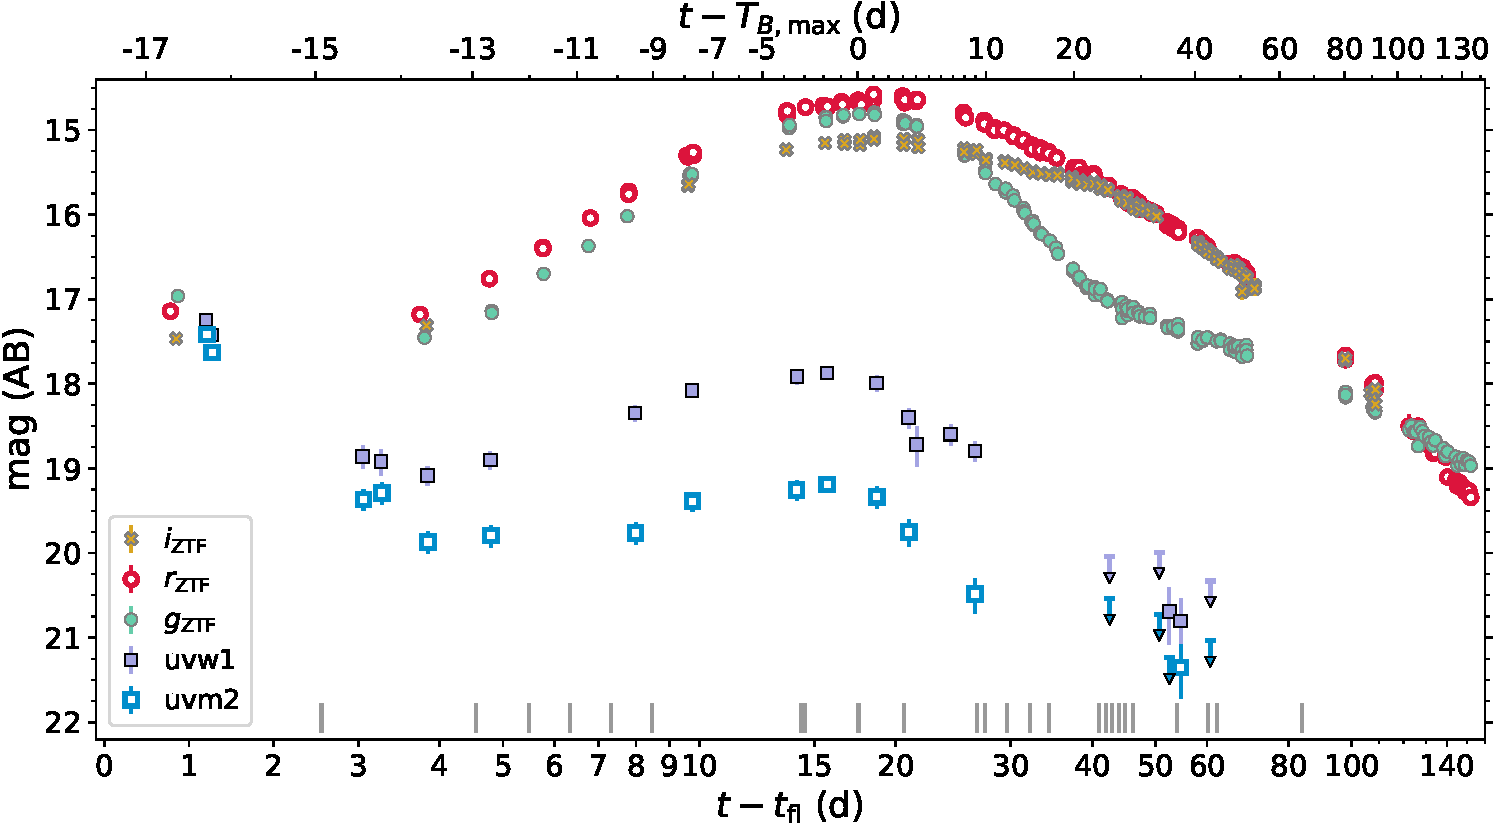
\includegraphics[width=6in]{./figures/P48_lc.pdf}
    %
    \caption{Photometric evolution of \sn, highlighting the initial decline
    observed in the light curve. \gztf, \rztf, and \iztf\ observations are
    shown as filled green circles, open red circles, and filled golden
    crosses, respectively. UVOT $uvw1$ and $uvm2$ are shown as filled and
    open squares, respectively. The lower axis shows time measured in
    rest-frame days relative to the time of first light, \tfl\ (see
    \S\ref{sec:phot}), while the upper axis shows time relative to the time
    of $B$-band maximum, \tbmax. Note that the horizontal axis is shown with
    a linear scale from $0\,\mathrm{d} \le t - t_\mathrm{fl} \le 3$\,d and a
    log scale for $t - t_\mathrm{fl} > 3$\,d. Vertical grey ticks show
    epochs of spectroscopic observations.}
    %
    \label{fig:p48}
\end{figure*}

The field of \sn\ was additionally observed by ZTF with nearly a nightly
cadence as part of the ZTF partnership Uniform Depth Survey (ZUDS;
D.~Goldstein et al., in prep.). Using images obtained as part of the ZUDS
program, we perform forced PSF photometry at the location of \sn\ following
the procedure described in \citet{Yao19}.\footnote{Images obtained as part of
the ZTF public survey have not been released, preventing us from applying our
forced-PSF measurements. We therefore only include forced-PSF measurements in
the analysis described herein, though we note that our measurements are
largely consistent with those provided in the public alerts.} The evolution
of \sn\ in the \gztf, \rztf, and \iztf\ filters is shown in
Figure~\ref{fig:p48}.

\subsection{Other Photometric Observations}\label{sec:swift}

Ultraviolet (UV) observations of \sn\ were obtained with the
Ultra-Violet/Optical Telescope (UVOT; \citealt{Roming05}) onboard the Neil
Gehrels Swift Observatory (hereafter \textit{Swift}; \citealt{Gehrels04})
following a time-of-opportunity request.\footnote{\textit{Swift} ToO
requests for \sn\ (\textit{Swift} Target ID: 13037) have been submitted by
D.~Hiramatsu, J.~Burke, and S.~Schulze.}
Pre-SN UVOT reference images are limited to the $uvw1$, $uvm2$, and $uvw2$
filters. As a result we cannot provide accurate estimates of the SN flux in
the \textit{Swift} $u$, $b$, and $v$ filters. We estimate the flux in the
$uvw1$, $uvm2$, and $uvw2$ filters using an aperture of size \steve{PPP}
pixels at the SN position, and subtract the flux measured using an identical
procedure in the pre-SN images \steve{Is this all correct?}. For clarity, we
only show the \textit{Swift} $uvw1$ and $uvm2$ light curves in
Figure~\ref{fig:p48}.\footnote{The $uvw2$ evolution is nearly identical to
$uvm2$. Furthermore, the red leak associated with the $uvw2$ filter (see
e.g., \citealt{Breeveld11}), in combination with the relatively red spectral
energy distribution of SNe\,Ia, make it very difficult to interpret $uvw2$
light curves of SNe\,Ia (see \citealt{Brown17} and references therein).
Therefore, unless otherwise noted, we exclude $uvw2$ measurements from the
analysis below.} \textit{Swift}/UVOT observations show that the initial
decline seen in the optical is even more dramatic in the UV.

While absolute flux measurements in the UVOT $u$, $b$, and $v$ filters are
not available, assuming the underlying flux from the host is constant, we
can estimate the time of $B$-band maximum, \tbmax, from the relative
$b$-band light curve. Using a second-order polynomial, we model the $b$-band
light curve near peak (including observations between JD$\,> \,$2,458,855.5
and JD$\,<\,$2,458,871.5). From this fit we estimate \tbmax$ =
$2,458,863.83$ \,\pm \,0.21$\,JD.

In parallel with the UV observations, \textit{Swift} observed \sn\ in the
X-rays with the X-ray Telescope \citep{Burrows05}. We do not detect variable
X-ray emission at the position of \sn, as is expected in SNe\,Ia (e.g.,
\citealt{Margutti12}). \todo{Note - if CSM interaction becomes the story of
this SN, then this paragraph needs to be revisited.}

\subsection{Optical Spectroscopy}

Spectroscopic observations of \sn\ were taken with a variety of telescopes
and instruments over multiple epochs beginning $\sim$2\,d after discovery
and continuing through $\sim$2\,months after \tbmax. An observing log is
listed in Table~\ref{tab:spectra}. The spectra were reduced using standard
procedures in \texttt{IDL}/\texttt{Python}/\texttt{Matlab}. The optical
spectral evolution of \sn\ is illustrated in Figure~\ref{fig:spec_evo}.

\begin{figure}
    \centering
    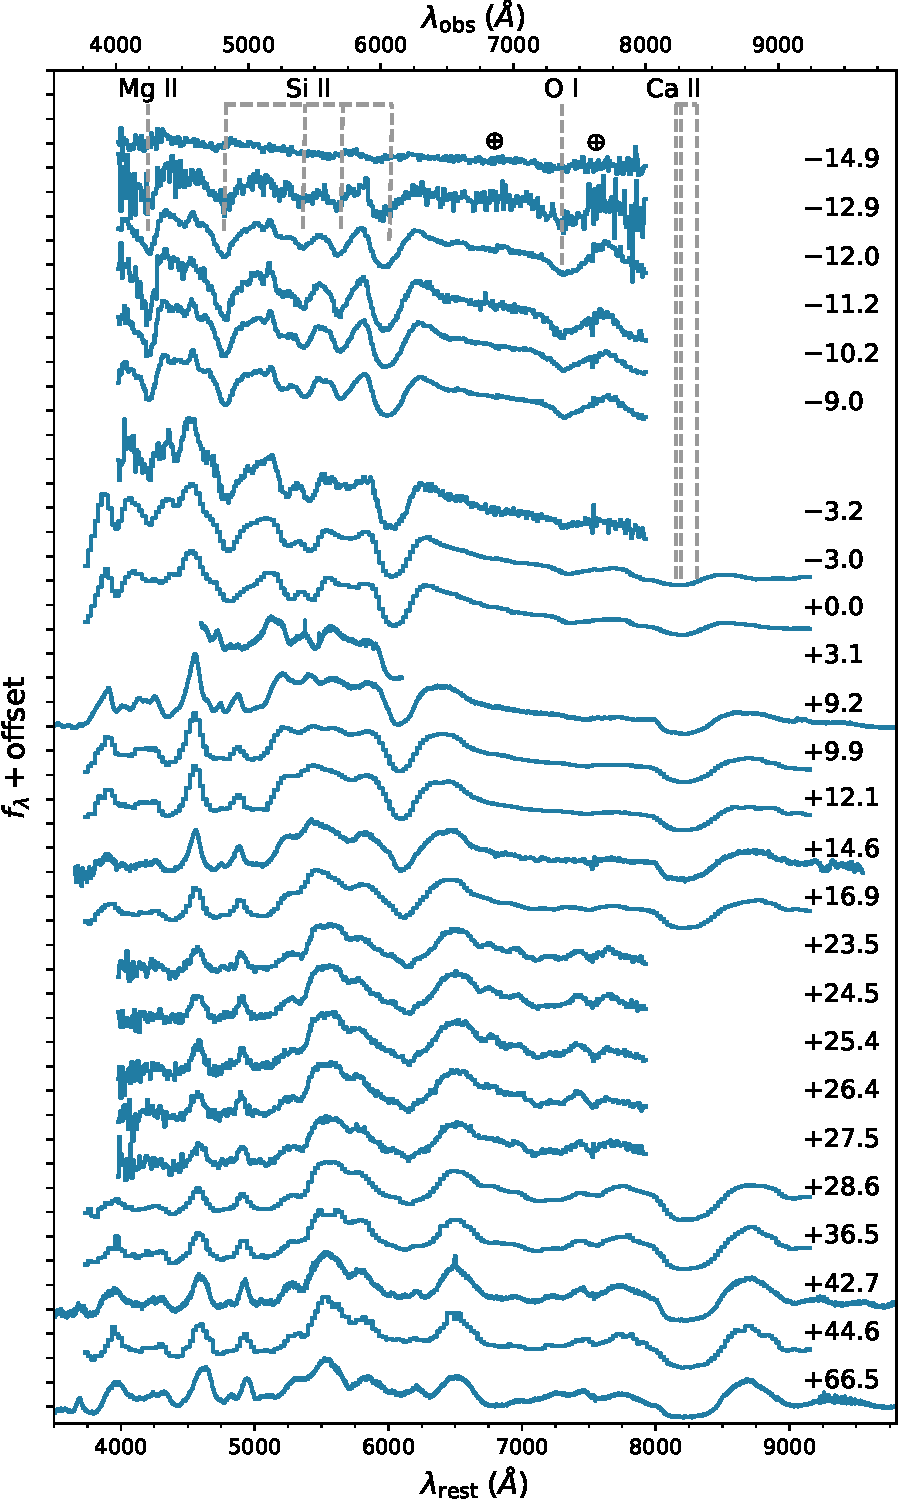
\includegraphics[width=3.35in]{./figures/spec_evo.pdf}
    %
    \caption{Observed spectral sequence of \sn. Spectra have been normalized
    by their median flux between 7200\,\AA\ and 7400\,\AA. The phase of each
    observation relative to \tbmax\ is shown to the right of the individual
    spectra. Prominent spectral features from intermediate mass elements are
    highlighted with vertical dashed lines. Some of the spectra show
    imperfect Telluric subtractions, giving rise to the non-smooth features
    around $\lambda_\mathrm{obs} \approx 7600$\,\AA.}
    %
    \label{fig:spec_evo}
\end{figure}

\section{NGC\,4441: the Host of \sn}\label{sec:host}

NGC\,4441 is the host galaxy of \sn. Sloan Digital Sky Survey (SDSS;
\citealt{York00}) spectroscopic measurements of the nucleus of NGC\,4441
yield a heliocentric-recession velocity of 2663\,\kms\ ($z_\mathrm{helio} =
0.00888$; \citealt{Abolfathi18}) and a \texttt{STARBURST} classification for
NGC\,4441. Morphologically, NGC\,4441 is classified as a peculiar,
weakly-barred, late-type lenticular galaxy (SABO$+$ pec;
\citealt{de-Vaucouleurs91}). SDSS images show a clear dust lane near the
center of the galaxy.

Using the 2M++ model of \citet{Carrick15}, we estimate a peculiar velocity
towards NGC\,4441 of $+328.6$\,\kms, which combined with the recession
velocity in the frame of the cosmic microwave background\footnote{See
\url{https://ned.ipac.caltech.edu/velocity_calculator}} (CMB,
$v_\mathrm{CMB} = 2770.6$\,\kms), yields a total recession velocity $=
3099.2 \pm 150$\,\kms. The final uncertainty in the total recession velocity
is dominated by systematic uncertainties in the 2M++ model. We also note
that the 2M++ estimate is consistent, to within $\sim$5\%, with the Virgo
and Great Attractor infall models of \citet{Mould00}. Adopting $H_0 =
73$\,\kms\,Mpc$^{-1}$, we estimate the distance to NGC\,4441 to be $42.5 \pm
2.1$\,Mpc, corresponding to a distance modulus of $\mu = 33.14 \pm
0.11$\,mag, where the uncertainty on $\mu$ is dominated by the uncertainty
in the peculiar velocity correction. We hereafter adopt 33.14\,mag as the
distance modulus to NGC\,4441.\footnote{\citet{Tully13} estimate a
significantly smaller distance to NGC\,4441 ($\mu = 31.43 \pm 0.14$\,mag; $D
= 19.0$\,Mpc) based on surface brightness fluctuation measurements from
\citet{Tonry01}. If NGC\,4441 is at this distance, then \sn\ peaks at $M_g
\approx -16.8$\,mag, which is significantly underluminous for a SN\,Ia.
Given that \sn\ has a normal rise time $t_\mathrm{rise} \approx 18$\,d
(\S\ref{sec:phot}), relatively normal spectra at peak (\S\ref{sec:spec}),
and produced $\sim$0.4\,$M_\odot$ of \radni\ (\S\ref{sec:tardis}), it is
highly unlikely that it is nearly a factor of 10 less luminous in the \gztf\
filter than normal SNe\,Ia. We therefore adopt the larger kinematic distance
to NGC\,4441.}
% \todo{Lots of different catalogs provide
% metallicity for SDSS galaxies, should we report on these results at all?
% Port Z = 0.04 and Granada Z ~0.01, and do not agree, firefly ~ 0.6 0r 0.2
% (solar?) depending on weighting, probably not a great idea} \fromkate{that's
% a reasonable spread in values but likely different calibrations. I don't
% know which one is best or the references for comparing this value to. }

We estimate the total redenning towards \sn\ to be small. There is
relatively little line of sight extinction due to the Milky Way, $E(B-V)
\approx 0.018$\,mag \citep{Schlafly11, Schlegel98}. Furthermore, we do not
find significant evidence for strong extinction in NGC\,4441.
Figure~\ref{fig:NaD} highlights the \ion{Na}{I} D absorption in the spectrum
of \sn\ due to gas in NGC\,4441 and the Milky Way from our
highest-resolution spectrum, $R \approx 4000$, obtained with Binospec+MMT.
The \ion{Na}{I} D absorption is weak, and we estimate a total equivalent
width (EW) $= 390$\,m\AA\ for NGC\,4441 and $220$\,m\AA\ for the Milky Way.
There is a systematic uncertainty of $\sim$10\% on each of these estimates
due to uncertainties in the continuum-fitting procedure. Assuming similar
properties for the dust in NGC\,4441 and the Milky Way, we scale the color
excess measurement for the Milky Way by the ratio of \ion{Na}{I} D EWs to
estimate $E(B-V) \approx 0.032$\,mag for \sn\ due to absorption in
NGC\,4441. This yields a total color excess towards \sn\ of $E(B-V) \approx
0.05$\,mag, which we adopt for the subsequent analysis in this study. We
note that this estimate is consistent, to within the uncertainties, with the
EW(\ion{Na}{I} D)--$E(B-V)$ relations presented in \citet{Poznanski12}.
Further supporting the claim of low extinction is the lack of a detection of
the \ion{K}{I} $\lambda\lambda$7665, 7699 interstellar lines or the diffuse
interstellar band at 5780\,\AA, which also serve as proxies for extinction
(e.g., \citealt{Phillips13}). \frommb{Maybe worth noting how estimate below
would change for peculiar dust as that seen in some SNe (e.g. SN 2014J,
Rv=1.4)}

\begin{figure}
    \centering
    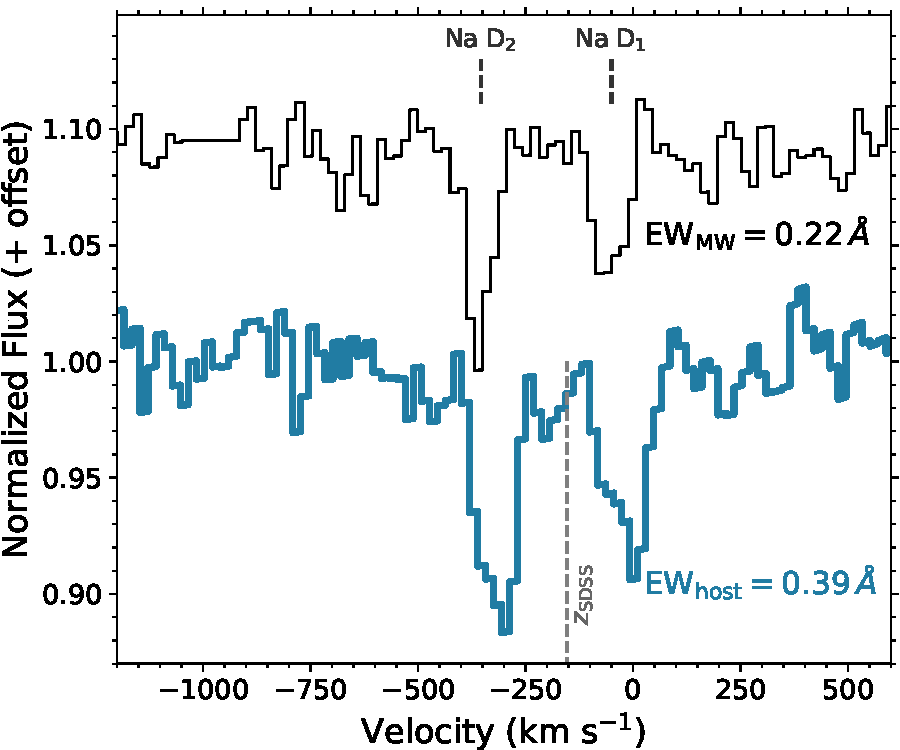
\includegraphics[width=3.35in]{./figures/NaD.pdf}
    %
    \caption{Zoom-in on our moderate resolution ($R \approx 4000$)
    MMT+Binospec spectrum of \sn\ highlighting absoprtion due to \ion{Na}{I}
    D in the host galaxy, NGC\,4441 (blue solid line), and the Milky Way
    (thin black line). The velocity scale is centered on the D$_1$ line in
    NGC\,4441, with the SDSS redshift shown via the vertical dashed line. No
    shift has been applied to the Milky Way lines. The \ion{Na}{I} D lines,
    which serve as a proxy for dust-obscuration along the line of sight
    (e.g., \citealt{Poznanski12,Phillips13}) are weak, indicating a
    relatively small amount of reddening.}
    %
    \label{fig:NaD}
\end{figure}



\section{Photometric Analysis}\label{sec:phot}

\subsection{The Time of First Light, \tfl}\label{sec:t_fl}

We estimate the time of first light, \tfl, for \sn\ following the procedure
described in \citet{Miller20}. Briefly, \citet{Miller20} model the early
emission from a SN Ia as a power-law in time, $f \propto (t -
t_\mathrm{fl})^\alpha$, where $f$ is the flux, $t$ is time, and $\alpha$ is
the power-law index. \tfl\ is assumed to be the same everywhere in the
optical, allowing us to simultaneously fit observations in each of the ZTF
filters.

An important caveat for \sn\ is that the observed early decline in the light
curve clearly does not follow the simple power-law model, and thus these
observations must be masked when performing the fit. We conservatively exclude
observations from the first two nights of ZTF detection from the fit (this
choice is conservative as it is unclear when the mechanism that powers the
initial bump in \sn\ no longer significantly contributes to the flux in the
\gztf\ and \rztf\ filters). From the fit we find \tfl$ = -17.5
\pm^{1.0}_{1.3}$\,d relative to \tbmax. We know that the time of explosion
must be $< -17.4$\,d based on the discovery detection in \citealt{Itagaki19},
and, by definition $t_\mathrm{fl} \ge t_\mathrm{exp}$, meaning a portion of
the posterior distribution for our model cannot be correct. We also find
$\alpha_g = 2.15 \pm^{0.49}_{0.36}$ and $\alpha_r = 1.91 \pm^{0.42}_{0.31}$.
These values are typical of the normal SNe Ia studied in \citet{Miller20}. If
we only exclude the first observation from the model fit we find significantly
different results with a rise time that increases by $\sim$5\,d and power-law
indicies that increase by $\gtrsim 1$. We note that such a long rise is
unlikely, however, as our spectroscopic models (see \S\ref{sec:tardis})
estimate the time of explosion, $t_\mathrm{exp}$, to be $\sim$17.9\,d prior to
\tbmax, fully consistent with our estimate of \tfl.

\fromkate{The rise time is long for its magnitude and stretch. From
\citet{Gonzalez-Gaitan12}, the risetime would suggest a high stretch event,
their fig. 12. Likely just the impact of the early component but worth
stressing. }

\subsection{Luminosity of the Initial UV/optical Flash}\label{sec:luminosity}

To estimate the luminosity and temperature of the intial UV/optical flash from
\sn, we model the broadband spectral energy distribution (SED) as a blackbody.
The assumed distance and reddening towards \sn\ are taken from
\S\ref{sec:host}. The ZTF optical and \textit{Swift} UV observations were not
simultaneous, so we therefore interpolate the optical light curves to estimate
the flux during the same epochs as \textit{Swift} observations. While SNe\,Ia
do not emit as pure blackbodies, this assumption is reasonable for the early
flash from \sn, which is distinctly different from normal SNe. Furthermore,
our intial spectrum of \sn\ shows a blue and nearly featureless continuum
largely consistent with blackbody emission.

Following interpolation to an epoch 1.24~rest-frame~d after \tfl\
($\mathrm{JD} = $2,458,847.43), we estimate a blackbody luminosity $L = (1.7
\pm ^{0.2}_{0.1}) \times 10^{42}$\,erg\,s$^{-1}$ and temperature
$T_\mathrm{eff} = 14.8 \pm^{0.9}_{1.2}$\,kK. This estimate represents a lower
limit to the peak luminosity of the initial flash, as the UV flux was already
decreasing at this time (\textit{Swift} obtained two sets of UV observations
separated by $\sim$90\,min during the first epoch of observations, and the
$uvm2$ and $uvm1$ flux is clearly decreasing during this time; see
Figure~\ref{fig:p48}). iPTF\,14atg, the other SN\,Ia to exhibit an early UV
flash, has an estimated flash luminosity of $\sim$3$ \times
10^{41}$erg\,s$^{-1}$, a factor of $\sim$5 less than for \sn, though we
caution that a direct comparison of these estimates requires the
\textit{Swift} observations to have been acquired at precisely the same epoch,
which is likely not the case.

At an epoch 3.15~rest-frame~d after \tfl, we estimate the luminosity and
temperature to have fallen to $L = (7.0 \pm ^{0.9}_{0.6}) \times
10^{41}$\,erg\,s$^{-1}$ and $T_\mathrm{eff} = 8.7 \pm^{0.5}_{0.4}$\,kK,
respectively. For this epoch we have excluded the $uvw2$ flux from the
blackbody model due to the significantly lower temperature, and known red leak
for that filter (see \S\ref{sec:swift}). This measurement of $t_\mathrm{eff}$
is consistent with spectral modelling at a similar epoch (see
\S\ref{sec:tardis}). If we assume that the early flash peaked 1\,d after \tfl,
and effectively ended 3\,d after \tfl\ (note -- both of these assumptions are
highly uncertain), then the initial flash emitted a total integrated energy of
$\sim$4$\times 10^{42}$\,erg.
% peak ~ 1.82e42; total = 1.82e42/2 + 2*7e41 + 1.12e+42

\subsection{Maximum Light and Decline}\label{sec:max_decline}

While the rise time and power-law indicies of \sn\ are similar to other normal
SNe Ia, the full photometric evolution does not resemble a normal SN\,Ia. \sn\
is somewhat underluminous ($M_{g,\mathrm{max}} \approx -18.5$\,mag), declines
rapidly ($\Delta m_{15}(g) = 1.30\pm^{0.01}_{0.02}$\,mag, uncertainties
represent the 68\% credible region), and does not exhibit a ``shoulder'' in
the \rztf\ or a secondary maximum in the \iztf\ light curves post-maximum
\fromkate{A plot of the light curves comparing to the Yao sample would be good
to compare brightness, secondary max and deltam15}. For context, of the 127
SNe\,Ia observed by ZTF and studied in \citet{Yao19}, only 1, ZTF18abclfee
(SN\,2018crl), a SN\,2002cx-like event, had a faster decline than \sn. The
underluminous, fast-declining evolution of \sn\ is broadly consistent with the
SN\,1991bg-like subclass of SNe Ia (e.g., \citealt{Taubenberger17}),
% and, according to the new photometric classification scheme presented in \citet{Ashall20}, \sn\ is consistent with  91bg-like SNe.
however, we show that \sn\ is spectroscopically distinct relative to 91bg-like
SNe (\S\ref{sec:spec}). We also find that standard SN Ia fitting techniques,
including \texttt{SALT2} \citep{Guy07} and \texttt{SNooPY} \citep{Burns11}, do
not provide good matches to the evolution of \sn. \fromkate{Explain briefly
why they don't work.}

\subsection{Color Evolution}

\sn\ is further distinguished from normal SNe Ia by its unusual color
evolution (Figure~\ref{fig:colors}). The top panel of Figure~\ref{fig:colors}
shows the \gztf$ - $\rztf\ evolution of 35 normal SNe Ia with ZTF observations
within 3\,d of \tfl\ (see \citealt{Bulla20}), with the color evolution of \sn\
over-plotted. \sn\ exhibits a prominent blue to red to blue, or ``red bump,''
evolution in the $\sim$week after \tfl. Similar red bumps are only seen in
$\sim$10\% of the ZTF sample \citep{Bulla20}. Furthermore, while normal SNe Ia
exhibit a large scatter in \gztf$ - $\rztf\ shortly after \tfl\ they evolve to
form a tight locus around \tbmax. \sn\ is redder at peak than each of the
normal SNe Ia in the \citet{Bulla20} sample, and it exhibits a far more rapid
decline in \gztf$ - $\rztf. In the $\sim$20\,d after \tbmax, the \gztf$ -
$\rztf\ color of \sn\ increases by $\sim$1.1\,mag, whereas the typical normal
SN Ia color only becomes $\sim$0.5\,mag redder over the same time frame.

\begin{figure}
    \centering
    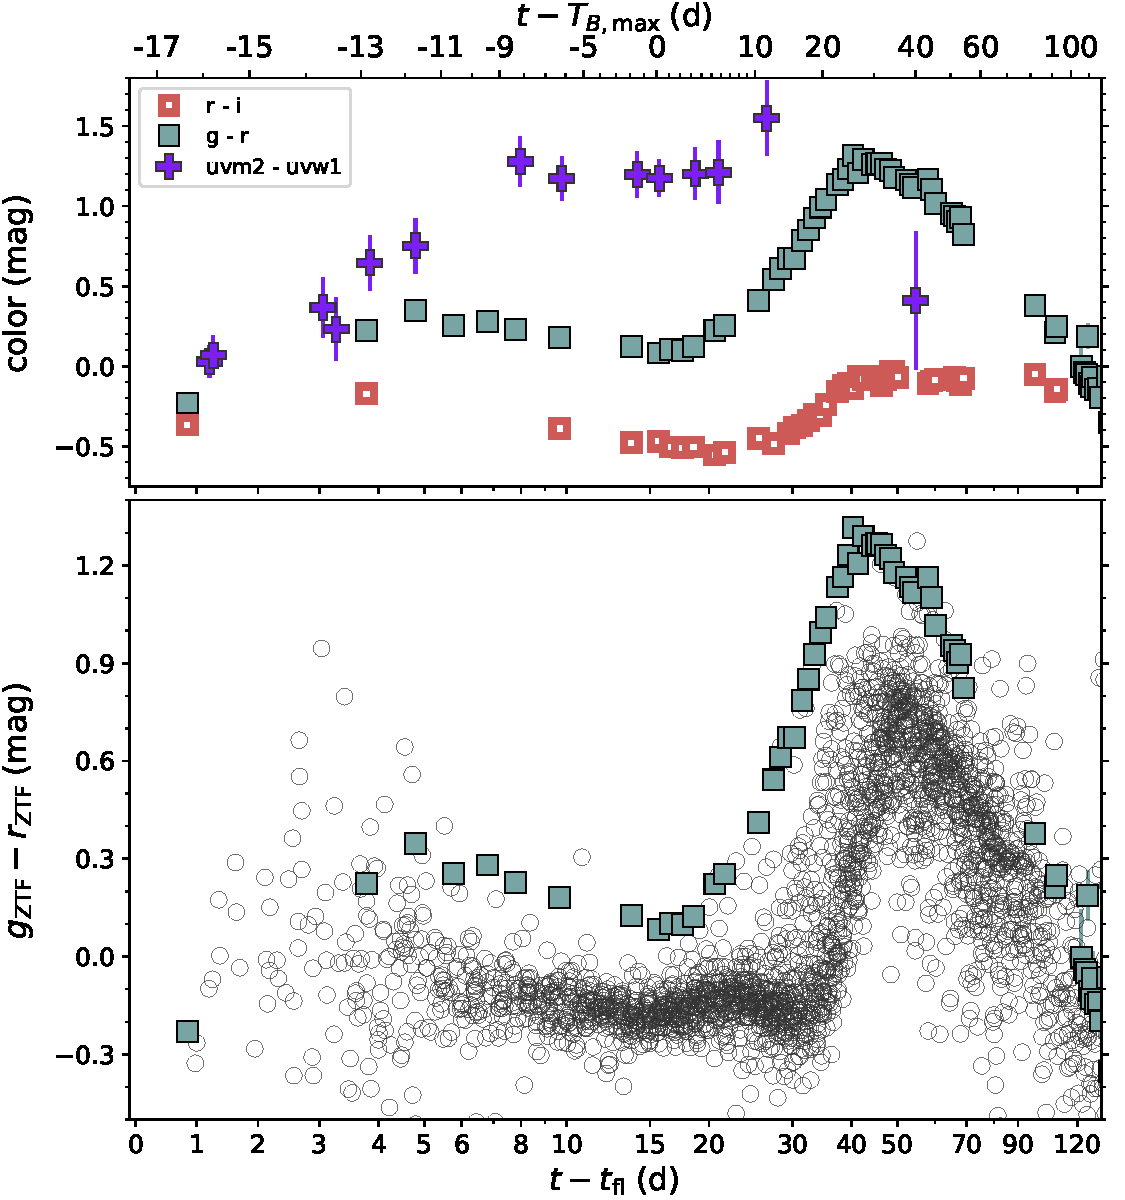
\includegraphics[width=3.35in]{./figures/P48_colors.pdf}
    %
    \caption{Photometric color evolution of \sn. \textit{Top}: \gztf$ -
    $\rztf\ evolution of \sn\ (solid green squares), corrected for the total
    line of sight extinction (see \S\ref{sec:host}), and compared with the
    evolution of 35 normal SNe Ia (open circles) observed within 3\,d of \tfl\
    by ZTF (from \citealt{Bulla20}). \sn\ is the reddest SN in the group, and
    it exhibits the fastest evolution to red colors post-\tbmax.
    \textit{Bottom}: the $uvm2 - uvw1$ (purple crosses), \gztf$ - $\rztf\
    (solid, green squares), and \rztf$ - $\iztf\ (open, red squares) color
    evolution of \sn. The ``red bump'' can clearly be seen in the optical.}
    %
    \label{fig:colors}
\end{figure}

The offset in the \gztf$ - $\rztf\ color evolution of \sn\ relative to normal
SNe\,Ia would be reduced if the reddenning towards \sn\ has been significantly
underestimated. A color excess of $E(B-V) \approx 0.25$\,mag, rather than the
0.05\,mag adopted in \S\ref{sec:host}, would roughly align the pre-\tbmax\
\gztf$ - $\rztf\ color of \sn\ with the tight locus seen in
Figure~\ref{fig:colors}. Such a correction would also bring the peak optical
brightness of \sn\ in line with normal SNe\,Ia [for $E(B-V) \approx
0.25$\,mag, $M_g \approx -19.25$\,mag and $M_r \approx -19.1$\,mag for \sn].

While the spectral appearance of \sn\ is similar to some normal SNe\,Ia (see
\S\ref{sec:spec_comp}), the observed rapid decline in the \gztf\ filter
provides strong evidence that \sn\ is not a normal luminosity SN\,Ia.
\citet{Phillips93} showed that in the optical SNe\,Ia follow a
brightness--width relation, whereby brighter explosions decline less rapidly.
Thus, with a typical peak in the optical, as would be implied with $E(B-V)
\approx 0.25$\,mag, the fast decline in \sn\ [$\Delta m_{15}(g) = 1.3$] would
be largely unprecedented.\footnote{As a reminder, \sn\ declines faster than
all but 1 SN in the sample presented by \citet{Yao19}.} We therefore conclude
that the color excess towards \sn\ is not underestimated, and that the SN is
instead intrinsically red in the optical.

% Such a large reddening would dramatically change the appearance of \sn\ in
% the UV. If we assume $E(B-V) \approx 0.25$\,mag, then the luminosity of the
% initial flash would be $\sim$8.7$\times 10^{42}$\,erg\,s$^{-1}$, more than a
% factor of 5 higher than what we estimated in \S\ref{sec:luminosity}.

% The bottom panel of Figure~\ref{fig:colors} shows the $uvm2 - uvw1$
% color evolution of \sn. At \tbmax, $uvm2 - uvw1 \approx 1.2$\,mag, making
% \sn\ one of the most UV blue SNe\,Ia at maximum light (e.g.,
% \citealt{Milne10,Brown17}). A color excess of $E(B-V) \approx 0.25$\,mag is
% equivalent to $E(uvm2 - uvw1) \approx 0.5$\,mag using the Fitzpatrick+
% (1999) extinction law, $R_V = 3.1$, and the effective wavelengths of the
% \textit{Swift} filters from \citet{Brown17} \frommb{I get 0.65 mag, maybe
% double-check?}. \fromkate{I did this calc, I've checked and using method and
% values listed, I get 0.5 mag for the uvm2-uvw1 colour} This results in a
% $uvm2 - uvw1 \approx 0.XXX$\,mag at \tbmax, making \sn\ the most UV blue
% SN\,Ia observed by \textit{Swift} \fromkate{this needs to be updated because
% none of the objects in Brown sample are corrected for extinction}.

Even if one ignores the striking initial bump in the light curve of \sn, we
can still conclude that \sn\ is not a normal SN Ia based on its other
photometric properties (e.g., relatively faint peak optical brightness,
moderately fast decline, lack of a near-infrared secondary maximum, and red
appearance at peak).

\section{Spectral Evolution of \sn}\label{sec:spec}

Optical spectra of \sn\ were obtained at phases from $-$14.9\,d (2.6\,d after
\tfl) to 66.5\,d after \tbmax. Details of the spectra are presented in
Table~\ref{} and the spectral evolution is shown in Figure~\ref{fig:spec_evo}.
The absorption features in \sn\ are typical of SNe\,Ia, including intermediate
mass elements (IMEs), primarily Si, Ca, and O, as well as iron-group elements
(IGEs).

\subsection{TARDIS Models}\label{sec:tardis}

To determine the structure of the ejecta and relative contributions of
different ions at early and maximum light phases, we have modelled the spectra
at $-$14.9\,d, $-12.0$\,d, and $+$0.0\,d using the 1D Monte Carlo radiative
transfer code \texttt{TARDIS} \citep{Kerzendorf14}. We note that
\texttt{TARDIS} assumes a single, sharp photosphere between the optically
thick and thin regions. Therefore, if there is a contribution to the spectrum
from an underlying quasi-blackbody (at early times this could be due to
interaction, for example; see Sect. XX), this will impact the ability of
\texttt{TARDIS} to fully reproduce the observations. Nevertheless, our models
should provide a reasonable approximation of the plasma state within the
ejecta. Parameters of our \texttt{TARDIS} models are given in
Table~\ref{tab:tardis}.

\begin{deluxetable*}{lcrrccc}
\tabletypesize{\scriptsize}
\tablewidth{0pt}
\tablecaption{\texttt{TARDIS} input parameters\label{tab:tardis}}
\tablehead{
\colhead{Date} &
\colhead{MJD} &
\colhead{Phase\tablenotemark{a}} &
\colhead{$t - t_\mathrm{exp}$\tablenotemark{b}} &
\colhead{$L$\tablenotemark{c}} &
\colhead{$v_\mathrm{boundary}$\tablenotemark{d} }&
\colhead{$T_\mathrm{boundary}$\tablenotemark{e} } \\
\colhead{(UT) }&
\colhead{} &
\colhead{(d)} &
\colhead{(d)} &
\colhead{($\log L_{\odot}$)} &
\colhead{(\kms) } &
\colhead{(K)}
}
\startdata
2019 Dec 31.277 & 58848.277 & $-14.9$ & 3.0 & 8.55 & 25,000 & 8173 \\
2020 Jan 03.217 & 58851.217 & $-12.0$ & 6.0 & 8.60 & 16,500 & 7925 \\
2020 Jan 15.392 & 58863.392 & $+0.0$ & 18.0 & 9.29 & 10,500 & 9696 \\
\enddata
\tablenotetext{a}{Rest-frame time relative to the time of $B$-band maximum,
\tbmax.}
\tablenotetext{b}{Rest-frame time relative to the \texttt{TARDIS} time of
explosion, $t_\mathrm{exp}$.}
\tablenotetext{c}{Emergent Luminosity.}
\tablenotetext{d}{Ejecta velocity at the inner boundary of the photosphere.}
\tablenotetext{e}{Temperature at the inner boundary of the photosphere. The
inner boundary temperature is not explicitly an input parameter for
\texttt{TARDIS}, it is derived from the luminosity, time since explosion,
inner boundary velocity, and iteratively updated throughout the simulation.}

\end{deluxetable*}

%%%Description of overall modelling results, velocities, features present, temperature. Then detailed discussion of Mg II vs Si III can be removed.
The first spectrum of \sn\ at $-$14.9\,d (2.6\,d after \tfl, 3.0\,d after
explosion) shows shallow features consistent with IMEs moving at extremely
high velocities ($>$\,20,000\,\kms, Figure~\ref{fig:spec_evo}). The
best-fitting \texttt{TARDIS} model is shown in Figure~\ref{fig:tardis}, along
with the contribution of individual elements to the spectral features. For
this model, we have assumed a uniform composition of O, Mg, Si, and S. Our
model demonstrates that the shallow absorption features observed at this phase
can be reproduced solely by IMEs (predominantly \ion{Si}{II}), and that the
presence of IGE is not required to match the data. Our model also confirms the
high velocities of the ejecta -- we find the spectral features and temperature
are best reproduced with a photospheric velocity of
$\sim$25,000\,\kms.

\begin{figure*}
    \centering
    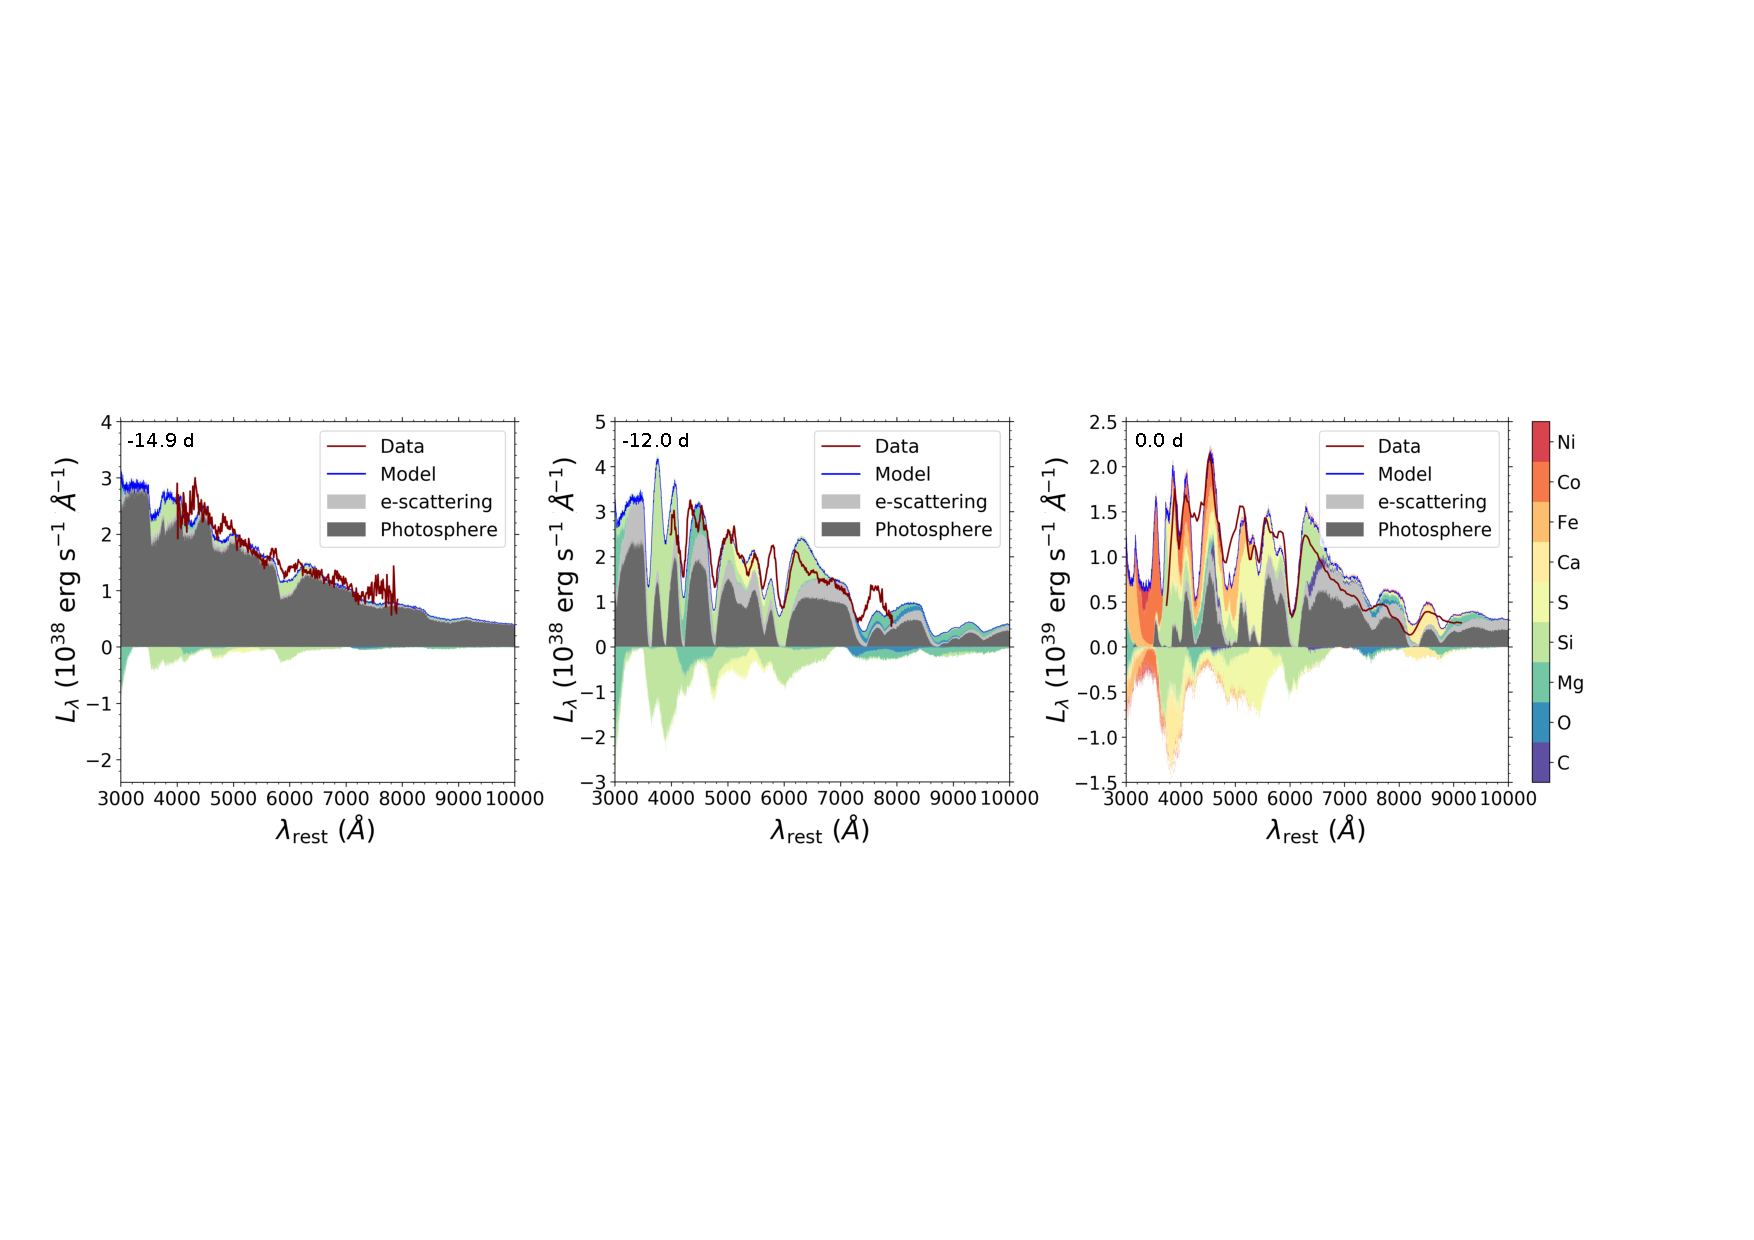
\includegraphics[width=\textwidth]{./figures/tardis.pdf}
    %
    \caption{Comparison of \texttt{TARDIS} models to \sn at $-$14.9\,d (left),
    $-12.0$\,d (middle), and $+$0.0\,d (right), relative to \tbmax. For each
    model, we colour code a histogram showing the contribution of each element
    to the spectroscopic features, based on the last element with which a
    Monte Carlo packet experienced an interaction. Those packets which
    underwent only electron scattering are shown in grey, while those that did
    not interact are shown in black. }
    %
    \label{fig:tardis}
\end{figure*}

Similarly, for the $-12.0$\,d spectrum we find that a model that does not
contain IGE above $\sim$16,500\,\kms\ reproduces the majority of the
spectroscopic features. Again, our model contains a uniform composition of O,
Mg, Si, and S, and is shown in Fig.~\ref{fig:tardis}. At this phase the model
suggests the photospheric temperature has not significantly changed, however
the features have become much more prominent. Compared to modelling of the
spectroscopically similar SN\,2002bo \citep{Stehle05} at the same epoch, see
below, we find \sn\ has a lower photospheric temperature ($\sim$8,000\,K,
compared to $\sim$9,500\,K for SN\,2002bo).

\magee{Can you confirm the following details about Carbon?} While the early
spectra of \sn\ are dominated by IMEs, we do not find evidence for
\ion{C}{II} absorption. This finding is supported by the fact that the
\texttt{TARDIS} models do not improve when C is added to the ejecta
composition.

Given that our maximum light spectrum occurs 12 days after our previous model
spectrum, we assume a composition for the inner ejecta
($\textless$16,500\,\kms\ ) similar to that found for SN\,2002bo
\citep{Stehle05}. A more detailed ejecta structure could be achieved through
modelling additional pre-maximum spectra, but is beyond the scope of the work
presented here. As shown in Fig.~\ref{fig:tardis}, our model is able to
broadly reproduce many of the features observed. Notable exceptions include
the features around $\sim$4200 and 4900\,\AA, which we attribute to Fe.
Better spectroscopic agreement could potentially be achieved if \sn\ had
a lower abundance of IGE within the inner ejecta relative to SN\,2002bo.

Overall, our \texttt{TARDIS} modelling demonstrates that \sn\ is consistent
with a low (or zero) fraction of IGE in the outer ejecta. Additionally, the
earliest phases show little change in temperature, as expected from the
colour evolution.

\frommark{Figure coming shortly}

\subsection{\ion{Si}{II} Evolution}\label{sec:SiII}

We have measured the velocity of the \ion{Si}{II} $\lambda$6355 absorption
feature following the procedure described in \S2.5 of \citet{Maguire14}. We
have also estimated the pseudo-equivalent widths (pEWs) of the \ion{Si}{II}
$\lambda\lambda$5972, 6355 features, allowing us to measure their ratio, also
known as the $\mathcal{R}($\ion{Si}{II}$)$; see \citet{Hachinger08} for the
updated definition relative to \citet{Nugent95}.

\begin{figure}
    \centering
    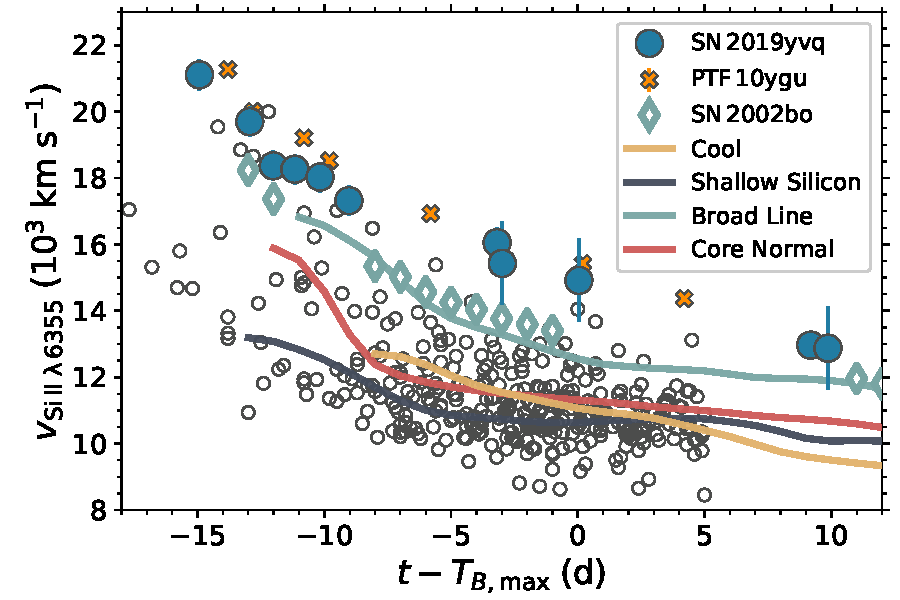
\includegraphics[width=3.35in]{./figures/vel_evolution.pdf}
    %
    \caption{Velocity evolution of \ion{Si}{II} $\lambda$6355\,\AA\
    absorption in \sn\ (large, filled circles). For comparison we also show
    the measurements for 264 SNe Ia observed by the Palomar Transient
    Factory (PTF) as open circles, with SN\,2010jn (PTF\,10ygu), the SN with
    the fastest moving ejecta in the PTF sample, highlighted via orange
    crosses. We additionally show the velocity evolution of SN\,2002bo, a SN
    that is very similar to \sn, as open diamonds. The median velocity
    evolution of each of the spectroscopic classes defined by
    \citet{Branch06} (Shallow Silicon, Core Normal, Broad Line, and Cool)
    are shown via solid lines. It is clear that \sn\ has exceptionally fast
    moving ejecta relative to typical SNe Ia.}
    %
    \label{fig:vel_evo}
\end{figure}

%%%Velocity and equivalent width measurements?
The velocity evolution of \ion{Si}{II} $\lambda$6355 is shown in
Figure~\ref{fig:vel_evo}, compared to measurements for the Palomar Transient
Factory (PTF) SN\,Ia sample from \citet{Maguire14} and the median velocity
evolution of SNe\,Ia belonging to the four different classes (Shallow
Silicon, Core Normal, Broad Line, and Cool) identified in
\citet{Branch06};\footnote{The velocity measurements are from
\citet{Blondin12}, while the method to determine the median velocity is
described in \citet{Miller18}.} hereafter, the \citeauthor{Branch06}~class.
The ion{Si}{II} $\lambda$6355 velocity is $\sim$15000 \kms.

At \tbmax, the pEW measurements for the \ion{Si}{II} $\lambda$6355 and
$\lambda$5972 features are $183\pm1$\,\AA, and $13\pm2$\,\AA, respectively,
unambiguously classifying \sn\ as a \citeauthor{Branch06}~Broad Line SN\,Ia.
\sn\ stands out in Figure~\ref{fig:vel_evo} with some of the highest
\ion{Si}{II} velocities that have ever been observed. Within the PTF sample,
only SN\,2010jn (PTF10ygu) exhibits a \ion{Si}{II} absorption velocity as
high as \sn\ at every phase in its evolution.

As first noted by \citet{Nugent95}, and later confirmed by
\citet{Hachinger08}, $\mathcal{R}($\ion{Si}{II}$)$ is a luminosity indicator,
with larger values of $\mathcal{R}($\ion{Si}{II}$)$ corresponding to lower
luminosities. This correlation is driven by the ionization balance of
\ion{Si}{II}/\ion{Si}{III}, with cooler objects having stronger \ion{Si}{II}
$\lambda$5972 features. In Figure~\ref{fig:r_evo}, we show the
$\mathcal{R}($\ion{Si}{II}$)$ of \sn\ as a function of time, compared to
SN\,2011fe, SN\,2002bo and the PTF spectral sample of \citet{Maguire14}. \sn\
has a similar $\mathcal{R}($\ion{Si}{II}$)$ evolution to SN\,2002bo from high
to low values from early times up to maximum light. This evolution is
different to that of SN\,2011fe and the majority of the PTF SN\,Ia sample.

\begin{figure}
    \centering
    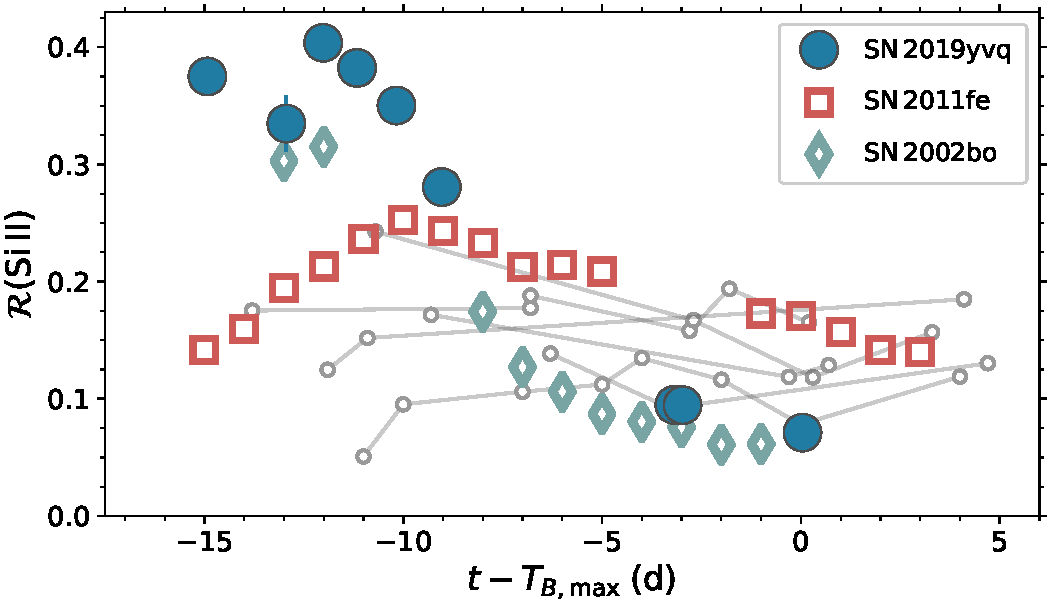
\includegraphics[width=3.35in]{./figures/R_evolution.pdf}
    %
    \caption{Evolution of the ratio of the pEW of \ion{Si}{II}
    $\lambda$5972\,\AA\ to \ion{Si}{II} $\lambda$6355\,\AA,
    $\mathcal{R}($\ion{Si}{II}$)$ in \sn\ (large, filled circles). For
    comparison we also show the measurements for 264 SNe Ia observed by the
    Palomar Transient Factory (PTF) as open circles. The velocity evolution
    of SN\,2002bo and SN\,2011fe are highlighted as open diamonds and open
    squares, respectively. \sn\ and SN\,2002bo exhibit an unusual inversion
    in $\mathcal{R}($\ion{Si}{II}$)$ as they evolve toward maximum light.}
    %
    \label{fig:r_evo}
\end{figure}

At face value, the $\mathcal{R}($\ion{Si}{II}$)$ evolution in
Figure~\ref{fig:r_evo} suggests that the effective temperature of \sn\
increases significantly as it rises to maximum light. The optical colors (see
Figure~\ref{fig:colors}), however, are nearly constant throughout this phase
while the UV$ - $optical colors clearly decline during the same period,
suggesting a decline in the effective temperature. The \texttt{TARDIS}
modelling also does not require a significant increase in temperature towards
maximum light from the temperature of $\sim$8,000\,K required at early times.
This stands in contrast to SN\,200bo, which increases in temperature from
$\sim$9,500\,K at $-12.9$\,d to $\sim$14,000\,K at maximum light
\citep{Stehle05}. This temperature is similar to \citeauthor{Branch06}~Core
Normal SNe, such as SN\,2011fe, which typically have temperatures of
$\sim$14,500--15,000\,K at maximum light \citep{Mazzali14}.

\citet{Benetti04} interpreted these competing effects as the result of
significant \ion{Si}{II} mixing in the ejecta of SN\,2002bo. Mixing or Si
production in the outermost layers of the ejecta would (i) lead to larger
\ion{Si}{II} velocities, (ii) produce \ion{Si}{II} line ratios that indicate
cool temperatures (because there is less radioactive material to heat the
ejecta), before eventually (iii) producing low values of
$\mathcal{R}($\ion{Si}{II}$)$ as the photosphere recedes through the ejecta
to higher temperature regions. This picture is consistent with the
\citet{Stehle05} models of SN\,2002bo. In those models, Si completely
dominates the species at velocities above $\sim$23,000\,\kms, while there is
very little ($\sim$1\%) IGE above a 1.35\,$M_\odot$ in radial mass
coordinates. The same explanation does not clearly apply to \sn, however, as
our \texttt{TARDIS} models do not show evidence for a significant increase
in the photospheric temperature at maximum light. Our \texttt{TARDIS} models
are, unlike SN\,2002bo, consistent with no IGEs in the outer layers of the
\sn\ ejecta. A possible explanation for the evolution of
$\mathcal{R}($\ion{Si}{II}$)$ in \sn\ is that as the photosphere receeds to
regions with more \radni, increased Si ionization occurs leading to a
relative decrease in \ion{Si}{II} $\lambda$5972 absorption despite
relatively small changes in the photospheric temperature.

\kate{and} \magee{This still seems like an unexplained puzzle to me...}

\subsection{Spectral Comparison}\label{sec:spec_comp}

%%%Comparison to other objects & Si II ratio
In Figure~\ref{fig:spec_comp}, we compare the spectral evolution of \sn\ to
two Broad-Line SNe, SN\,2002bo and SNe\,2010jn, and two Cool SNe, SN\,1986G
and SN\,2004eo \citep{Cristiani92,
Benetti04,Pastorello07,Silverman11,Hachinger13,Maguire14} at four phases,
pre-maximum, maximum, $\sim$1 week post maximum, and $\sim$6 weeks post
maximum. The evolution of \sn\ and SN\,2002bo is remarkably similar at all
phases. The only significant difference between the two is the absorption
trough at $\sim$4800\,\AA\ in the pre- and maximum-light spectra. This
feature, which is typically attributed to a combination of \ion{Fe}{II},
\ion{Fe}{III}, and \ion{Si}{II}, is extremely narrow in \sn. This is in
agreement with the \texttt{TARDIS} modelling results where no Fe is required
in the outer ejecta of \sn\ to match the observed spectra at early times.
SN\,2010jn, which exhibits large \ion{Si}{II} velocities like \sn, shows
weaker IME absorption and stronger IGE absorption than \sn. While the
\citeauthor{Branch06}~Cool SNe\,1986G and 2004eo feature lower velocities than
\sn, there is strong agreement in the relative \ion{Si}{II} line strengths of
SN\,1986G and the earliest spectra of \sn.

% The left panel of Figure~\ref{fig:spec_comp} also shows the spectrum of
% SN\,1986G, a \citet{Branch06} Cool SN that is sometimes referred to as
% ``transitional'' given its intermediate properties between normal SNe\,Ia and
% the sub-luminous SN\,1991bg-like population (e.g., \citealt{Pastorello07}).
% The \ion{Si}{II} line ratios, and narrow $\sim$4800\,\AA\ feature in SN\,1986G
% are similar to \sn, confirming the cool nature of the photosphere at this
% early epoch. The $-12.0$\,d spectrum of \sn\ additionally shows a weaker blue
% line in the \ion{S}{II} ``W'' absorption feature at $\sim$5400\,\AA, which is
% also consistent with cool temperatures \citep{Nugent95}.

\begin{figure*}
    \centering
    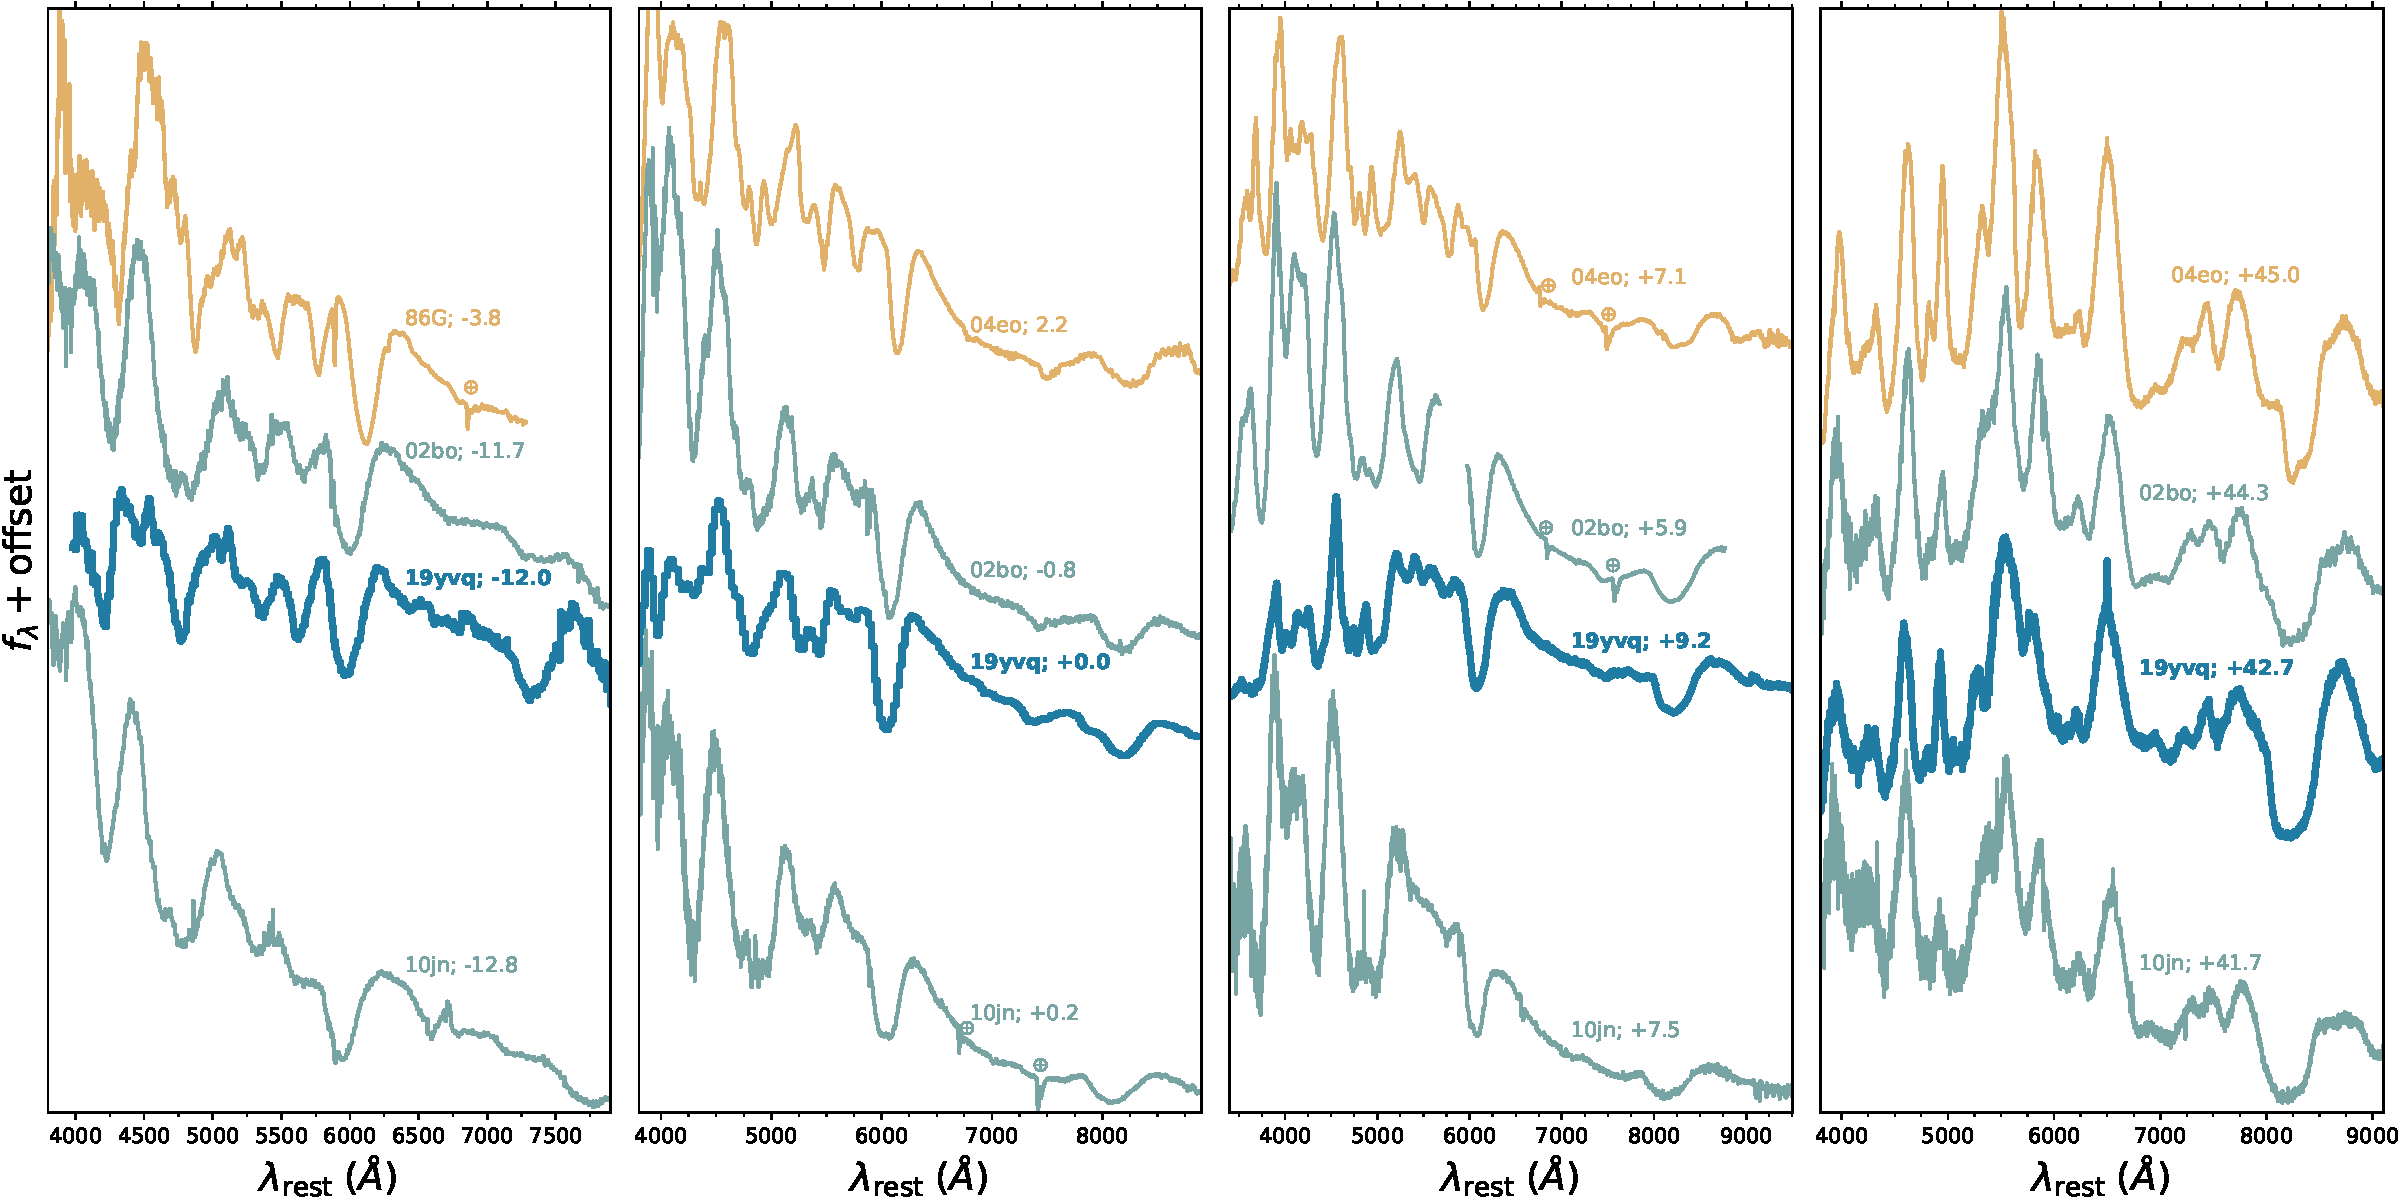
\includegraphics[width=7.25in]{./figures/spec_comp_extinction.pdf}
    %
    \caption{Spectral comparison of \sn\ to \citeauthor{Branch06}~Broad Line
    and Cool SNe\,Ia. All spectra have been corrected for the total
    line-of-sight extinction with adopted $E(B-V)$ values of 0.9\,mag,
    0.38\,mag, 0.39\,mag, 0.109\,mag, and 0.05\,mag for SNe\,1986G
    \citep{Phillips87}, 2002bo \citep{Stehle05}, 2010jn \citep{Hachinger13},
    2004eo \citep{Pastorello07}, and \sn\ (this work), respectively.
    \textit{Left panel}: pre-maximum spectra showing the similarity of \sn\
    and SN\,2002bo. While the expansion velocities in the Cool SN\,1986G
    spectrum are considerably lower than those in the Broad Line SNe, the
    relative ratios of the \ion{Si}{II} features are similar to \sn.
    \textit{Second panel}: Comparison of \sn\ to the Broad Line SNe\,2002bo
    and SN\,2010jn. These SNe all feature nearly identical maximum-light
    spectra. By this phase, the relative strength of the \ion{Si}{II}
    absorption features is no longer similar to \citet{Branch06} Cool SNe, as
    illustrated by SN\,2004eo. \textit{Third panel}: $\sim$1 week post-maximum
    spectra. \textit{Fourth panel}: Transitional phase spectra. Comparison
    spectra have been downloaded from WISeREP \citep{Yaron12}, with spectra
    for individual SNe from the following sources: SN\,1986G --
    \citet{Cristiani92}, SN\,2002bo -- \citet{Benetti04,Silverman11},
    SN\,2010jn (PTF\,10ygu) -- \citet{Hachinger13,Maguire14}, SN\,2004eo --
    \citet{Pastorello07}. \todo{Should this be 2 figures?}}
    %
    \label{fig:spec_comp}
\end{figure*}

The maximum-light spectra shown in the second panel of
Figure~\ref{fig:spec_comp} reveal a much higher luminosity/temperature for
\sn, as the \ion{Si}{II} $\lambda$5972\,\AA\ absorption has nearly disappeared
around \tbmax\ (see discussion of $\mathcal{R}($\ion{Si}{II}$)$ in
\S\ref{sec:SiII}). The appearance of \sn, SN\,2002bo, and SN\,2010jn are all
similar at this epoch, with the exception of the 4800\,\AA\ feature mentioned
above. SN\,2004eo has a similar appearance to \sn, though it has lower
velocities and cooler temperatures (as traced by \ion{Si}{II} $\lambda$5972).

The $+9.2$\,d spectrum of \sn, shown in the third panel of
Figure~\ref{fig:spec_comp}, shows absorption due to IGE. Additional
differences between \sn\ and SN\,2002bo can be seen at this phase. There is
stronger absorption in \sn\ blueward of \ion{Ca}{II} H\&K, and the \ion{S}{II}
``W'' absorption feature is still present in \sn\ and it cannot be identified
in SN\,2002bo or SN\,2010jn. SN\,2004eo maintains an appearance that is
somewhat similar to \sn, though as before, the temperatures are cooler and the
velocities lower.

Spectra obtained $\sim$6 weeks after maximum light are shown in the fourth
panel of Figure~\ref{fig:spec_comp}. By this time, as the SNe are
transitioning into a nebular phase, the appearance of each spectrum is similar
modulo some minor differences in the relative line strengths of different
features.

\frommb{I wonder if somewhere in Section 3 we should point out that
low-luminosity and high velocities are unprecedented (see data in Figure 11 of
Polin et al. 2019)...} \fromabi{I agree. This is unlike any of the data point
I could get my hands on and I think this is worth stating, because it is hard
to come up with something that has little Ni (low luminosity) but has enough
kinetic energy to boost to these velocities.}

\kate{do you want to say anything about \ion{Ca}{II}?}

\section{A Physical Explanation for \sn}\label{sec:models}

\fromkate{I've been looking at the violent merger models of Kromer+ 2013, 2016 to explain SN 2010lp and iPTF\,14atg. They don't explain the early flash but they can explain the red colours, the lack of secondary max, the intermediate peak brightness, lack of IGE in the early spectra and the high velocity and broad Si II lines. Early UV flash could come from CSM in the surrounds of the merger. I think this model is worth mentioning.}\frommark{Also related is the DOM scenario of e.g. Levanon \& Soker 2019}

The most striking feature of \sn\ is the observed UV/optical peak that occurs
shortly after discovery (Figure~\ref{fig:p48}). Any model to explain \sn\ must
account for this highly unusual feature. A UV decline in the early phase of a
SN\,Ia has previously only been observed in a single event, iPTF\,14atg
\citep{Cao15}. Clearly resolved ``bumps'' in the early optical emission of
SNe\,Ia are also rare, having only been seen in a few events: SN\,2017cbv
\citep{Hosseinzadeh17} and SN\,2018oh \citep{Shappee19,Dimitriadis19}.

\sn\ features other properties, in addition to an intial peak $\sim$17\,d
prior to \tbmax, that separate it from normal SNe\,Ia. A good model should be
able to explain the following characteristics of \sn:
%
\begin{enumerate}
    \item The early UV/optical ``flash'' (Figure~\ref{fig:p48}).
    \item The moderately faint peak in the optical (\S\ref{sec:max_decline}). 
    \item The relatively fast optical decline (\S\ref{sec:max_decline}). 
    \item The red optical colors at all epochs (Figure~\ref{fig:colors}). 
    \item The lack of IGE in the early spectra (\S\ref{sec:tardis}).
    \item The evolution in \RSiII\ (\S\ref{sec:SiII} and Figure~\ref{fig:r_evo}).
    \item The large photospheric velocities (Figure~\ref{fig:vel_evo}).
    \item The lack of C in the early spectra (\S\ref{sec:tardis})
\end{enumerate}
%

As noted in \S\ref{sec:phot}, the photometric evolution of \sn\ is similar to
subluminous 91bg-like SNe, however, the spectra are missing the hallmark
\ion{Ti}{II} absorption trough associated with 91bg-like SNe
\citep{Filippenko92}. Furthermore, around \tbmax, \RSiII\ is small in \sn,
whereas 91bg-like SNe feature large values of \RSiII\ (e.g.,
\citealt{Nugent95,Branch09}). Similarly, while the spectral appearance and
evolution of \sn\ is similar to SN\,2002bo, and other
\citeauthor{Branch06}~Broad Line SNe, the photometric properties are entirely
different. SN\,2002bo features a relatively slow decline [$\Delta{m}_{15}(B) =
1.13$\,mag] with a clear secondary maximum in the $I$ band \citep{Benetti04},
which is wholey different from what is observed in \sn.

If we otherwise ignore the early flash, several of the remaining features
(2--6) in the list above can be understood if the explosion that gave rise to
\sn\ produced a relatively small amount of \radni\ that is strongly confined
to the inner regions of the SN ejeta. A low \radni\ yield could explain the
underluminous light curve and red colors, while a highly stratified ejecta
structure could explain the lack of IGE in the early spectra as the IGE would
not have been mixed to these outer layers. Furthermore, with a highly
stratified ejecta composition, the photosphere would transition somewhat
rapidly from \radni-poor to \radni-rich, resulting in a significant change in
the luminosity/temperature of the ejecta along the lines of what we see in the
evolution of \RSiII.

\citet{Magee20} developed a suite of models featuring different \radni\
structures within the SN ejecta. These models were compared to early
observations of SNe\,Ia to see which ones replicate what is observed in
nature. Generally, it is found that highly stratified models do not match the
early evolution of normal SNe\,Ia \citep{Magee20}. However, when we model the
early evolution of \sn\ using the models of \citet{Magee20}, we find that the
observations are best matched by highly stratified models, as shown in
Figure~\ref{fig:Ni_mixing}. For this modelling we have excluded the first two
epochs of ZTF observations, as we consider the mechanism that produces the
early UV flash to be different from the standard \radni\ decay that powers
most SNe\,Ia. That the (normal) rising portion of the \sn\ light curve is best
matched by stratified models strengthens the support for this interpretation.
We note, however, that \citet{Magee20} demonstrate that the time of first
detection can dramatically alter the inferred model properties and it is
unclear which epochs (if any) should be excluded. Nevertheless, a stratified
ejecta is also consistent with our spectroscopic analysis (see
\S\ref{sec:tardis}).

\begin{figure}
    \centering
    \includegraphics[width=3.35in]{./figures/preliminary_Ni_mixing.png}
    %
    \caption{PRELIMINARY PRELIMINARY PRELIMINARY}
    %
    \label{fig:Ni_mixing}
\end{figure}

On their own, a low-\radni\ yield and highly stratified ejecta fail to explain
the blue UV/optical flash seen in \sn. A large number of scenarios have been
proposed to explain early ``bumps'' or ``flashes'' in SNe\,Ia light curves,
including: interaction between the SN ejecta and WD binary
companion \citep{Kasen10a}, interaction between the SN ejecta and
circumstellar material (e.g., \citealt{Dessart14,Piro16}), shock cooling
following the shock breakout from the surface of the WD (e.g.,
\citealt{Piro10,Rabinak11}), double detonation explosions (e.g.,
\citealt{Noebauer17,Polin19}), and extended clumps of \radni\ in the SN ejecta
(e.g., \citealt{Shappee19,Dimitriadis19}). We discuss these models and their
ability to replicate observations of \sn\ below.\footnote{We do not discuss
shock breakout models as our initial detection of \sn\ occurred at $M_g
\approx -16.3$\,mag. A progenitor radius of $\sim$10$\,R_\odot$ is needed to
explain such a high luminosity \citep{Piro10,Rabinak11}, which we consider
implausible for a WD.}

\subsection{Companion Interaction}

For SD progenitors of SNe\,Ia, the SN ejecta will shock on the surface of the
non-degenerate companion giving rise to a short-lived transient in the days
after explosion. \citet{Kasen10a} provided models for the appearance of this
interaction, which is primarily dependent upon the binary separation of the
system (assuming Roche lobe overflow for the non-degenerate companion). The
observed emission following the ejecta-companion collision is dependent upon
the orientation of the system at the time of explosion relative to the line of
sight \citep{Kasen10a}.

An analytic formulation for the luminosity and effective temperature of the
emission from the companion shock is given in Equations~22 and 25 in
\citet{Kasen10a}. \citet{Brown12} provide an analytic function to approximate
the fractional decrease in the observed flux as a function of the orientation
of the system. We combine equations from \citet{Kasen10a} and \citet{Brown12}
to model the early emission from \sn\ as ejecta-companion collision. We assume
the interaction emits as a blackbody, and that the electon scattering opacity
$\kappa_e = 0.2$\,cm$^{2}$\,g$^{-1}$ (as in \citealt{Kasen10a}). Assuming
$z_\mathrm{SN} = 0.0094$, $E(B-V)_\mathrm{MW} = 0.018$\,mag, and
$E(B-V)_\mathrm{host} = 0.032$\,mag, we compare observed flux measurements
with those predicted by the \citet{Kasen10a} model in epochs with MJD$\,<
58849.2$ (i.e., the first $\sim$2.5\,d after discovery when emission from the
companion interaction is significantly brighter than the luminosity due to
radioactive decay).\footnote{Given that \sn\ is an unusual SN, we make no
assumptions about the ``normal'' SN emission due to radioactive decay of
\radni. The companion-interaction model should therefore
\textit{underestimate} the observed flux as there will be a growing
contribution due to radioactive decay with time.} The model parameters,
including: the companion separation, $a$, the mass of the ejecta,
$M_\mathrm{ej}$, the velocity of the ejecta, $v_\mathrm{ej}$, the angle
between the observer, the SN, and the companion, $\theta$, and the time of
explosion, $t_\mathrm{exp}$ are constrained via a Gaussian likelihood and flat
priors (see Table~\ref{tab:priors}) using an affine-invariant
\citep{Goodman10} Markov Chain Monte Carlo (MCMC) ensemble sampler
\citep{Foreman-Mackey13}.

\begin{figure}
    \centering
    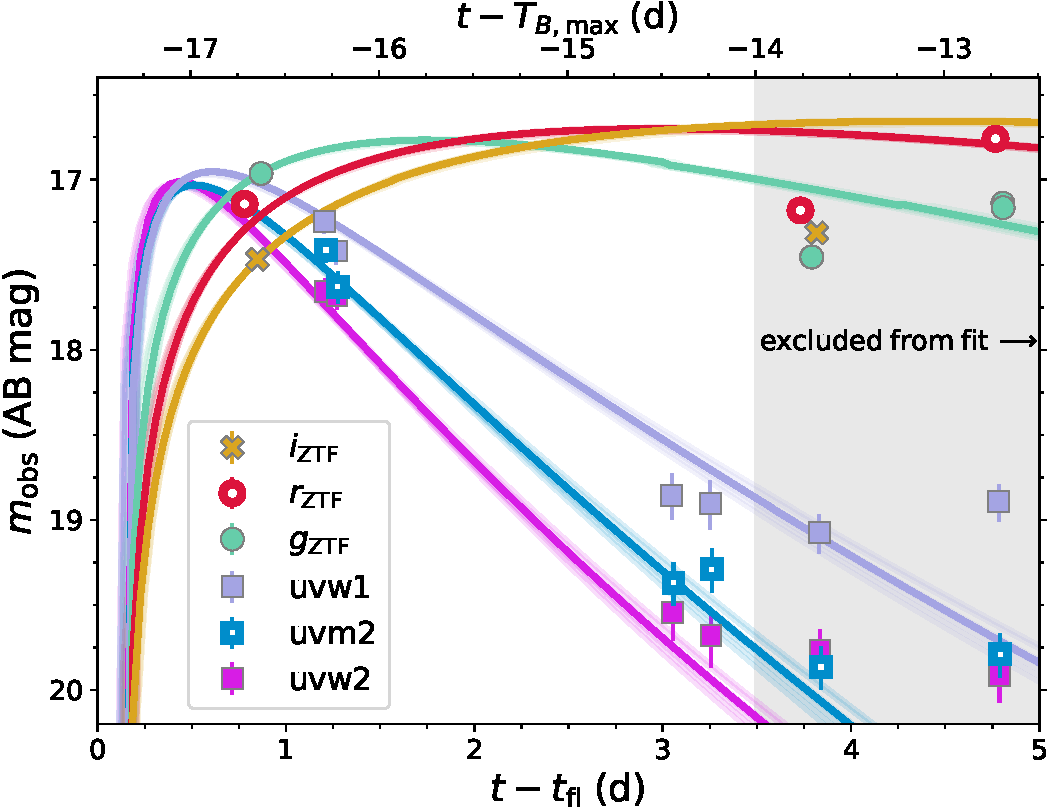
\includegraphics[width=3.35in]{./figures/sn_companion_models.pdf}
    %
    \caption{SN ejecta-companion interaction models compared with the
    UV/optical observations of \sn. Observation symbols are the same as
    Figure~\ref{fig:p48} (solid magenta squares show \textit{Swift} $uvw2$
    observations that are not shown in Figure~\ref{fig:p48}). Solid lines show
    companion interaction model predictions in each filter (the lines have the
    same colors as the corresponding symbols for each passband). The maximum a
    posteriori model is shown via the single bold lines, while other random
    draws from the posterior are shown as thin transparent lines. The shaded
    area shows observations that are excluded from the model fit. The
    overprediction of the optical flux $\sim$13.7\,d prior to \tbmax\ suggests
    that companion interaction does not explain the early flash in \sn\ (see
    text).}
    %
    \label{fig:companion}
\end{figure}

The results of this procedure are shown in Figure~\ref{fig:companion}, where
it is clear that the model presented in \citet{Kasen10a} does an adequate job
of explaining the early UV/optical emission from \sn. We find marginalized
posterior values of $a = 9.1 \pm 0.7 \times 10^{11}$\,cm, $M_\mathrm{ej} = 1.0
\pm 0.3\,M_\odot$, $v_\mathrm{ej} = 2.2 \pm^{0.5}_{0.3} \times 10^{4}$\,\kms,
$\theta = 34 \pm^{28}_{24} \deg$, and $t_\mathrm{exp}(\mathrm{MJD}) = 58845.83
\pm 0.05$ (all uncertainties are 68\% credible regions). Examination of a
corner plot of the posterior samples shows that $M_\mathrm{ej}$ is largely
unconstrained, while $v_\mathrm{ej}$ is degenerate with $\theta$ and $a$ is
degenerate with $t_\mathrm{exp}$. 

While the interaction models roughly approximate the SN emission in the
$\sim$3\,d after explosion, they significantly \textit{overestimate} the flux
immediately after the fitting window as shown in Figure~\ref{fig:companion}.
This problem is exacerbated by the fact that the models do not include
emission associated with radioactive decay, meaning the true discrepancy
between what is predicted and what is observed is even larger than what is
shown in Figure~\ref{fig:companion}. If we extend the fitting window to
include the optical observations obtained $\sim$13.75\,d before \tbmax, the
interaction models still overpredict the optical flux at this epoch. This
overprediction of the optical flux poses a challenge for the companion
interaction scenario; an inability to simultaneously match both UV and optical
observations has been noted for other SNe\,Ia with early bumps or linear rises
\citep{Hosseinzadeh17,Miller18}.

For this reason, we do not favor the ejecta-companion interaction
interpretation for \sn. \citet{Kasen10a} notes several assumptions and
approximations in the derivation of the equations used to estimate the
emission from the companion shock. It is possible that the inclusion of more
detailed physics, or additional complexity in the analytic formulation of the
models,\footnote{For example, \citet{Kasen10a} points out that the derived
equation for the luminosity of the shock interaction does not account for the
advected luminosity that would be seen in the observer frame.} could better
reconcile companion interaction models with \sn. Such improvements are beyond
the scope of this paper, leading us to explore other explanations for the
early flash.

\subsection{Ni Clumps in the SN Ejecta}

SN\,2018oh was observed with an exquisite 30\,min cadence by the
\textit{Kepler} spacecraft and showed a clearly delineated linear rise in
flux followed by a ``standard'' $t^2$ power-law $\sim$4\,d after \tfl. Models
with extended clumps of \radni\ just below the WD surface have been proposed
as a possible explanation for the initial linear rise in SN\,2018oh
\citep{Shappee19,Dimitriadis19}. The models considered in \citet{Shappee19}
and \citet{Dimitriadis19}, which build on the work of \citet{Piro16}, only
cover the first $\sim$10\,d after explosion and assume relatively simple grey
opacities. To further investigate this possibility, Magee \& Maguire (2020)
recently performed more detailed radiative transfer calculations for SNe\,Ia
with extended clumps of \radni. They then compared these models to SN\,2018oh
and SN\,2017cbv, another event with a clearly resolved bump in the early
light curve \citep{Hosseinzadeh17}.

\begin{figure}
    \centering
    \includegraphics[width=3.35in]{./figures/colour.pdf}
    %
    \caption{PRELIMINARY PRELIMINARY PRELIMINARY}
    %
    \label{fig:Ni_bullet}
\end{figure}

For \sn\ we follow the procedure in Magee \& Maguire (2020) to model the early
flash and rise of the SN. Briefly, we exclude the first two epochs of optical
detections in ZTF, and identify the best-fit model to the later evolution of
the SN from the grid of models created in \citet{Magee20}, see
Figure~\ref{fig:Ni_mixing}. Following the generation of this ``baseline''
model, we add clumps of \radni\ to the outer layers of the SN ejecta, and
perform full radiative transfer calculations using TURTLS \citep{Magee18}. We
find that a model with a 0.02~$M_{\rm{\odot}}$ clump of \radni\ best matches
the light curve shape of \sn, as shown in Figure~\ref{fig:Ni_bullet}. While a
clump of \radni\ can broadly replicate the observed flash in the optical, like
Magee \& Maguire (2020), we find that the extended clump of \radni\
dramatically alters the appearance of the SN at maximum light in a way that is
incompatible with observed spectra. We therefore conclude that Ni clumps
cannot explain the early flash seen in \sn.

\subsection{Double Detonation Models}

WDs that accrete a thin shell of He can explode via a ``double detonation''
whereby explosive burning in the He shell drives a shock into the C/O core of
the WD igniting explosive C burning, which leads to a detonation that
disrupts the entire WD (e.g., \citealt{Nomoto82,Nomoto82a,Woosley94}). Such
explosions are even possible in C/O WDs that are well below the Chandrasekhar
mass (see \citealt{Fink07, Fink10} and references therein).

Recent models of double detonation explosions presented in \citet{Polin19}
show that such explosions can replicate several of the peculiar properties of
\sn, including: the early UV/optical flash, a blue to red to blue color
transition, the low optical luminosity, red colors at maximum, a lack of
unburned C in the spectra, and a lack of IGE in the early spectra. However,
there is no single model that replicates each of these individual features.

The appearance of double detonation SNe\,Ia is effectively determined by two
properties: the mass of the C/O core of the WD and the mass of the He shell.
High mass WDs ($\gtrsim 1.1\,M_\odot$) produce large ($\gtrsim 1$4,000\,\kms)
photospheric velocities, while low mass WDs ($\lesssim 0.9\,M_\odot$) produce
less \radni\ and therefore are underluminous, relative to normal SNe\,Ia, at
peak \citep{Polin19}. That we see both of these features in \sn\ presents a
challenge for the \citet{Polin19} double detonation models. Furthermore,
thick He shells ($M_\mathrm{He} \gtrsim 0.05\,M_\odot$) produce more
pronounced UV/optical flashes shortly after explosion, particularly in
conjunction with lower mass WDs, while thin He shells ($M_\mathrm{He}
\lesssim 0.02\,M_\odot$) produce a more extreme color inversion in the days
after explosion.

We have attempted to model the evolution of \sn\ as a double detonation
explosion, following the procedure in \citet{Polin19}. We have specifically
focused on matching the photometric evolution (as noted above no models
create high-velocity ejecta and underluminous optical peaks), with particular
attention to the colors during the early flash and at maximum light. We find
that a model with $M_\mathrm{WD} = 0.92\,M_\odot$ C/O core and a
$M_\mathrm{He} = 0.04\,M_\odot$ He shell best match \sn, as shown in
Figure~\ref{fig:double_det}.

\begin{figure}
    \centering
    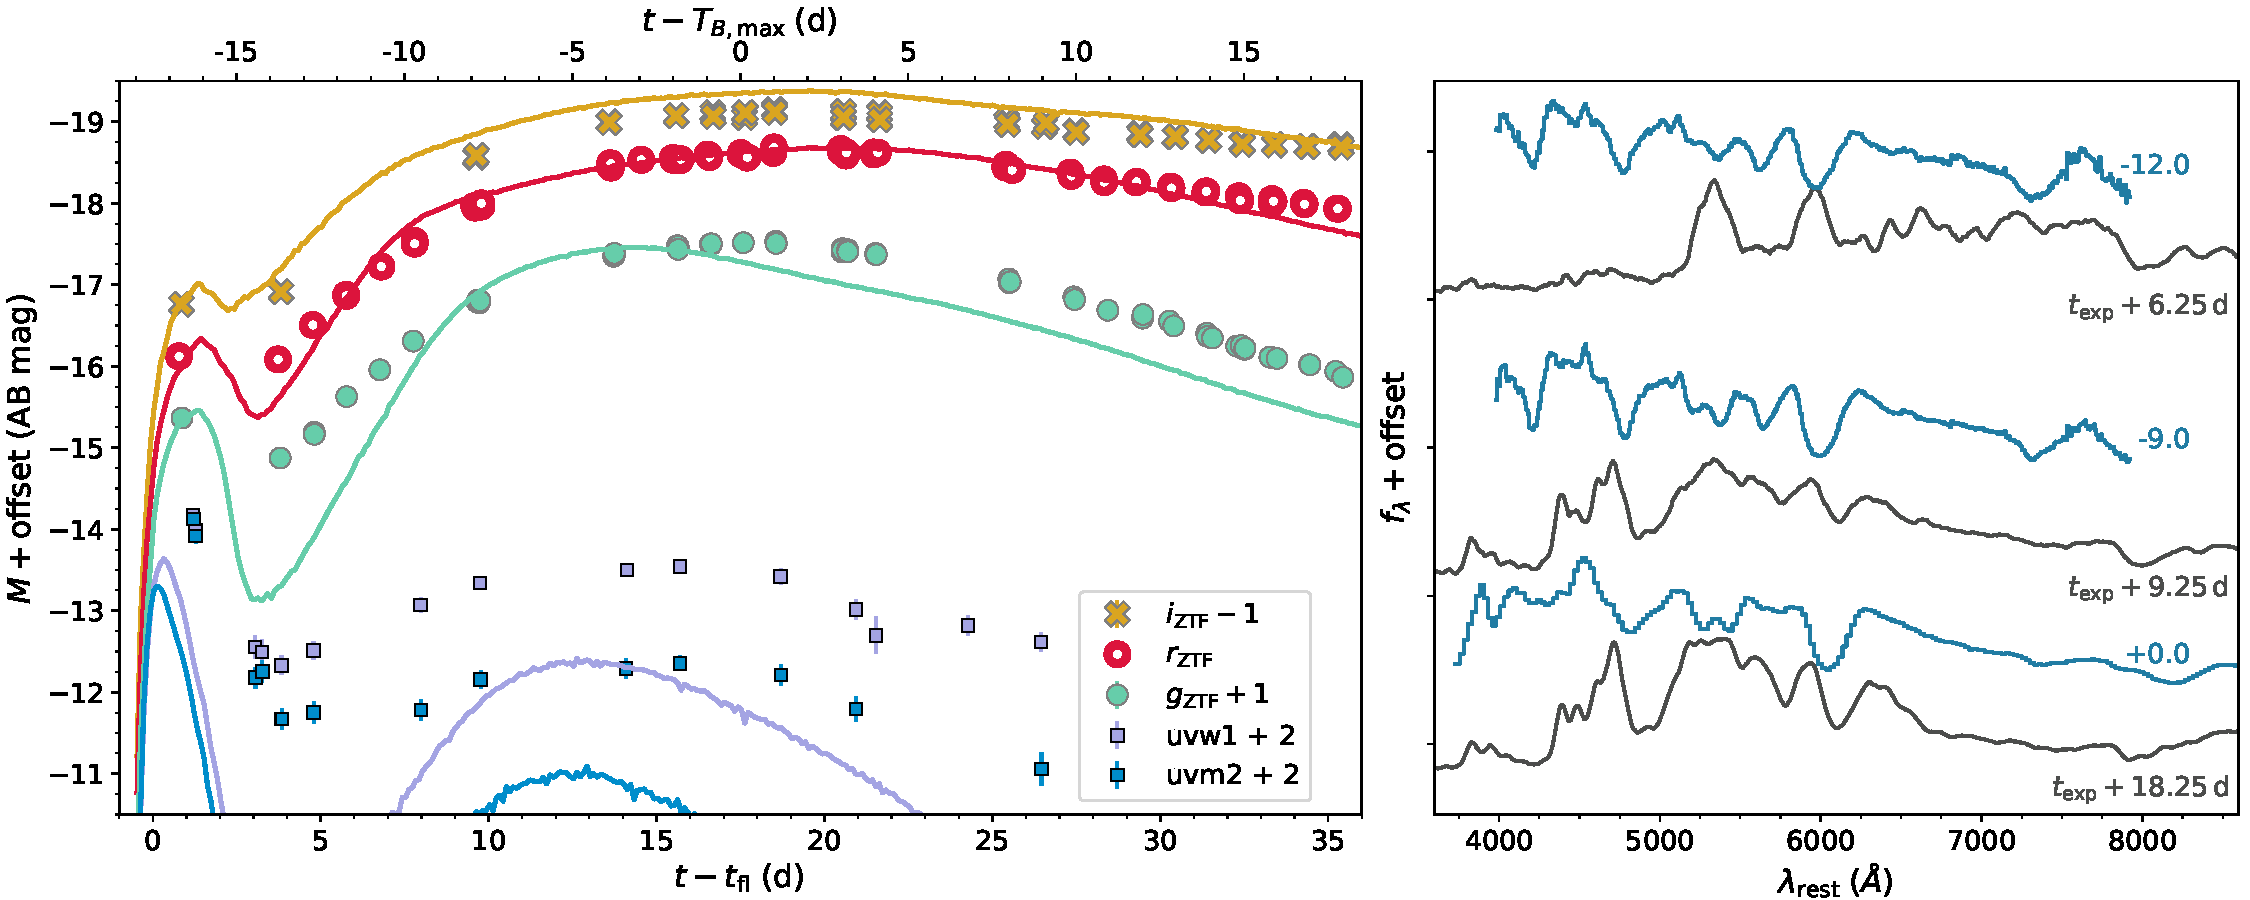
\includegraphics[width=3.35in]{./figures/double_det.pdf}
    %
    \caption{Comparison of \sn\ to a dobule detonation model with a C/O core
    mass $M_\mathrm{WD} = 0.92\,M_\odot$ and He shell mass $M_\mathrm{He} =
    0.04\,M_\odot$. Symbols are the same as Figure~\ref{fig:p48}. The double
    detonation model provides a good match to the \rztf\ evolution, though
    the flux in the \gztf\ and \iztf\ bands is under- and over-predicted,
    respectively.}
    %
    \label{fig:double_det}
\end{figure}

While this model adequately matches the evolution of \sn\ in the \rztf\
filter, the predictions in the \gztf\ and \iztf\ bands do not match what is
observed. The double detonation model also severely underpredicts the flux in
the UV. Synthesized spectra from the double detonation models also do not
match what is observed in \sn. The model spectra are dominated by \ion{Si}{II}
absorption, and show high-velocity absorption due to \ion{O}{I} and
\ion{Ca}{II}, similar to \sn. For this model, however, the \ion{Si}{II}
velocities are too slow, the \ion{Si}{II} $\lambda$5972 absorption is too
strong, the \ion{S}{II} absorption too weak, and there is a strong
\ion{Ti}{II} absorption trough blueward of $\sim$4400\,\AA\ (see e.g.,
Figure~8 in \citealt{Polin19}). Nuclear burning in the He shell creates heavy
elemnts in the outermost ejecta of double detonation explosions, leading to
deep \ion{Ti}{II} troughs and other blanketing in the blue-optical. As was the
case for models with extended clumps of \radni, the lack of such absorption in
\sn\ poses a challenge for the double detonation model.

It is possible that improvements in the double detonation models could lead to
better agreement with \sn. For instance, the nuclear reaction networks and 1D
models in \citet{Polin19} always burn the He shells to nuclear statistical
equilibrium. It is not unreasonable to think that 2D or 3D models, with a more
sophisticated nuclear reaction network, would create more IMEs and less IGEs
in the He shell. This could explain the lack of IGEs and strong \ion{Si}{II}
absorption seen in the early spectra, while less IGEs in the outer layers
would also reduce some of the blanketing seen around maximum light. This would
lead to less reprocessing of blue photons, perhaps creating better agreement
between the models and the \gztf\ and \iztf\ observatiions. \abi{please
provide additional details here. Also - any ideas about improving match in the
UV?}

\subsection{Violent Mergers and Circumstellar
Interaction}\label{sec:merger_csm}

\citet{Piro16} show that circumstellar material in the vicinity of a WD at the time of explosion can give rise to 


\section{Rate of Thick He Shell Double Detonation Events}\label{sec:rates}

\textbf{This may not actually be a thick shell}

\aam{Use rough numbers from CLU and simple binomial calculation}

\section{Discussion and Conclusion}\label{sec:conclusions}

\todo{be clever}

\acknowledgements

A.A.M.~is funded by the Large Synoptic Survey Telescope Corporation, the
Brinson Foundation, and the Moore Foundation in support of the LSSTC Data
Science Fellowship Program; he also receives support as a CIERA Fellow by the
CIERA Postdoctoral Fellowship Program (Center for Interdisciplinary
Exploration and Research in Astrophysics, Northwestern University).

This work is based on observations obtained with the Samuel Oschin Telescope
48-inch and the 60-inch Telescope at the Palomar Observatory as part of the
Zwicky Transient Facility project. ZTF is supported by the National Science
Foundation under Grant No. AST-1440341 and a collaboration including Caltech,
IPAC, the Weizmann Institute for Science, the Oskar Klein Center at Stockholm
University, the University of Maryland, the University of Washington,
Deutsches Elektronen-Synchrotron and Humboldt University, Los Alamos National
Laboratories, the TANGO Consortium of Taiwan, the University of Wisconsin at
Milwaukee, and Lawrence Berkeley National Laboratories. Operations are
conducted by COO, IPAC, and UW.

MMT Observatory access was supported by Northwestern University and the
Center for Interdisciplinary Exploration and Research in Astrophysics (CIERA).

We acknowledge the use of public data from the \textit{Swift} data archive.

\software{
          \texttt{astropy} \citep{Astropy-Collaboration13},
          \texttt{scipy} \citep{2020SciPy-NMeth}, 
          \texttt{matplotlib} \citep{Hunter07},
          \texttt{pandas} \citep{McKinney10},
        %   \texttt{emcee} \citep{Foreman-Mackey13},
        %   \texttt{corner} \citep{Foreman-Mackey16},
          \texttt{SALT2} \citep{Guy07},
          \texttt{sncosmo} \citep{Barbary16}
          }

%% For this sample we use BibTeX plus aasjournals.bst to generate the
%% the bibliography. The sample63.bib file was populated from ADS. To
%% get the citations to show in the compiled file do the following:
%%
%% pdflatex sample63.tex
%% bibtext sample63
%% pdflatex sample63.tex
%% pdflatex sample63.tex

\bibliography{/Users/adamamiller/Documents/tex_stuff/papers}
\bibliographystyle{aasjournal}

%% This command is needed to show the entire author+affiliation list when
%% the collaboration and author truncation commands are used.  It has to
%% go at the end of the manuscript.
%\allauthors

%% Include this line if you are using the \added, \replaced, \deleted
%% commands to see a summary list of all changes at the end of the article.
%\listofchanges

\begin{deluxetable*}{ccccc}
\tabletypesize{\scriptsize}
\tablewidth{0pt}
\tablecaption{Log of Spectroscopic Observations for SN~2019yvg.\label{tab:spectra}}
\tablehead{
\colhead{Date (UT)}&
\colhead{MJD}&
\colhead{Phase$^{*}$}&
\colhead{Telescope+Instrument}&
\colhead{Range}\\
\colhead{}&
\colhead{(days)}&
\colhead{(days)}&
\colhead{}&
\colhead{(\AA)}}
\startdata
31 Dec 2019 &  58848.273298   &    &  LT+SPRAT$^{*}$ &  4000--9000?   \\
03 Jan 2020 &     &     &  LT+SPRAT$^{*}$ &  4000--9000   \\
04 Jan 2020 &     &     &  LT+SPRAT &  4000--9000   \\
12 Jan 2020 &     &     &  LT+SPRAT &  4000--9000   \\
12 Jan 2020 &     &     &  LT+SPRAT  &  4000--9000   \\
15 Jan 2020 &     &     &  P60+SEDM$^{**}$ &  4000--9000   \\
18 Jan 2020 &     &     &  P60+SEDM &  4000--9000   \\
24 Jan 2020 &     &     &  MMT+Binospec$^{***}$ &  4000--9000   \\
25 Jan 2020 &     &     &  Keck+LRIS$^{****}$ &  4000--9000   \\
27 Jan 2020 &     &     &  P60+SEDM  &  4000--9000   \\
29 Jan 2020 &     &     &  NOT+ALFOSC$^{******}$ &  4000--9000   \\
01 Feb 2020 &     &     &  P60+SEDM &  4000--9000   \\
\enddata
\tablenotetext{*}{Liverpool Telescope}
%\tablenotetext{**}{}
%\tablenotetext{***}{}
\end{deluxetable*}



\end{document}